% Build: latexmk -pdf main.tex
\documentclass[aps,prx,reprint,superscriptaddress,nofootinbib]{revtex4-2}

\usepackage{graphicx}
\usepackage{amsmath,amssymb}
\usepackage{xcolor}
\usepackage{booktabs}
\usepackage{tikz}
\usetikzlibrary{arrows.meta,positioning,calc}
\usepackage{hyperref}
\hypersetup{colorlinks=true,linkcolor=blue!60!black,citecolor=blue!60!black,urlcolor=blue!60!black}

% ./ first so an arXiv/journal tarball with the figures alongside main.tex
% builds unchanged; ../results/ is the in-repo location.
\graphicspath{{./}{../results/}}

\newcommand{\Fe}{F_{\mathrm{e}}}

\begin{document}

\title{Native gates or nothing: the condition for a qudit advantage\\
in uncorrected quantum algorithms under decoherence}

\author{John Doxaras}
\email{john@ai-employee.cloud}
\thanks{AI Employee, \url{https://ai-employee.cloud}}
\affiliation{AI Employee, Athens, Greece}

\date{\today}

\begin{abstract}
Whether qudits buy resilience against decoherence is a recognized open
question: prior work compares algorithms by noiseless resource counts,
or error-correcting codes, which have no problem instance to compress.
We simulate Shor order finding, eigenstate phase estimation, and Grover
search as bare, uncorrected circuits---the regime of near-term
demonstrations---on qubit, qutrit, and ququint registers (with a
demo-size $d=7$ check) under two decoherence
channels---a ladder channel calibrated to published per-level transmon
coherence data and a depolarizing channel representative of trapped-ion
qudits---three entangling-gate cost models, and registers to
$5.3\times10^{5}$ Hilbert dimensions (19.0 qubit-equivalents). One condition governs all three algorithms: \emph{qudits
outperform qubits only with a native two-qudit entangling gate whose
cost grows no faster than linearly in $d$}. Gates compiled by two-level
decomposition forfeit the advantage in every case tested but
one---Shor at $d=3$ under per-particle noise, where width compression
alone survives the depth surcharge; whether linear cost suffices is
set by the level and structure of the operating dephasing---the
advantage holds on per-particle and refocused-ladder hardware,
free-evolution ladder dephasing splits the linear-cost cells, and
unmitigated Zeeman-structured dephasing reverses the verdict
outright. Along
the way we identify a number-theoretic confound---grid alignment of the
phases $s/r$---that reverses naive cross-dimension Shor comparisons and
predicts the winner in every biased instance tested (three instances
$\times$ two noise models), and we reduce the mechanism to a
quantitative law: accumulated channel damage fixes end-state fidelity
on a single exponential across algorithms and bases, with amplitude
${\approx}1$ and $R^2=0.97$--$0.99$ (the first-order expectation; in
log fidelity the law holds within a factor of two until states
approach their $1/\!\dim$ floor); the algorithm enters only through
its decoder's error tolerance, which we reduce to an exact
number-theoretic law verified outcome-for-outcome against the decoder.
The qubit branch of our predictions is anchored on hardware: the
shallow compiled circuit reproduces its predicted success band on a
commercial trapped-ion processor ($0.617\pm0.007$ vs $0.60$--$0.70$),
pinning the device's effective depolarizing strength at its measured
per-gate infidelity.
\end{abstract}

\maketitle

% =====================================================================
\section{Introduction}
\label{sec:intro}

Quantum hardware is not binary by nature. Transmons, trapped ions,
nitrogen-vacancy centers, and molecular spins all expose more than two
usable levels, and processors that exploit them as qudits now exist on
several
platforms~\cite{ringbauer2022,blok2021,goss2022,low2023,gardill2020,chiesa2024}.
The theoretical case for higher dimensions is old and, at the level of
structure, strong: fault-tolerant stabilizer constructions close cleanly
in prime dimension~\cite{gottesman1998} and the discrete phase-space
structure is cleanest in odd prime dimension~\cite{gross2006};
magic-state distillation protocols exist in every prime
dimension~\cite{campbell2012}, with thresholds and efficiencies that
keep improving with $d$ (within congruence classes mod 3, for primes up
to 17)~\cite{campbell2014}; and qudit memory thresholds rise under
abstract noise models~\cite{marks2017}. A base-$d$ register also compresses algorithms:
at matched problem size it needs $\log_2 d$ times fewer carriers and a
proportionally shorter schedule.

Whether any of this survives \emph{physical} decoherence---in which
higher levels of a real device decay and dephase faster than lower
ones---is a question the literature has flagged repeatedly and not
answered. Campbell noted that ``in physical systems one may also see
noise rise with $d$. Such features depend subtly on the details of the
underlying physics''~\cite{campbell2014}; Marks \emph{et al.} point to
the ``increased degrees of freedom that can be coupled to the
environment'' and call whether such noise can be kept sufficiently
small ``an interesting question for experimental
implementations''~\cite{marks2017}; Pavlidis and Floratos, citing qubit
evidence that order finding tolerates truncation of small QFT
rotations~\cite{barenco1996,nam2012}, conjecture ``a similar
robustness'' for qudits but leave its investigation
open~\cite{pavlidis2017}; and the recent qudit review of Kiktenko
\emph{et al.} lists ``the investigation of the impact of noise within
the discussed schemes'' as an open problem~\cite{kiktenko2023}.
Comparisons \emph{across} dimensions still treat noise indirectly:
entangling-gate counts as a noise
proxy~\cite{nikolaeva2021,kiktenko2023}, analytic coherent-error
bounds~\cite{bocharov2016}, or the qualitative argument that fewer
carriers means less local noise~\cite{wang2020}. Noisy qutrit circuit
simulations exist~\cite{gokhale2019,gustafson2022}, but always at
$d=3$ against a qubit baseline; no study has compared several prime
dimensions on full algorithms under channels calibrated to measured
per-level coherences, or followed such a comparison to scale. A claim
that qudit phase-estimation error decreases exponentially with
$d$---attributed by the review of Wang \emph{et
al.}~\cite{wang2020} to a conference contribution of Parasa and
Perkowski~\cite{parasa2011}, whose slides state it for the
algorithm's intrinsic failure probability at fixed precision (the full
text we were unable to obtain)---concerns the noiseless algorithm and
has, to our knowledge, never been tested against a noise model.

This paper answers the question quantitatively at the algorithm level.
We simulate Shor order finding~\cite{shor1997}, eigenstate quantum
phase estimation (QPE)~\cite{kitaev1995}, and Grover
search~\cite{grover1996} on qubit ($d=2$), qutrit ($d=3$), and ququint
($d=5$) registers, under two decoherence channels chosen to bracket real
hardware---an anharmonic-ladder channel calibrated to published
per-level transmon coherence measurements
\cite{peterer2015,goss2022,blok2021,tripathi2024,wang2024}, and a
per-particle depolarizing channel representative of trapped-ion
qudits~\cite{ringbauer2022,low2023}---under three entangling-gate cost
models spanning native gates, the measured trapped-ion
$2(d{-}1)$ M{\o}lmer--S{\o}rensen cost~\cite{ringbauer2022}, and
$O(d^2)$ two-level decomposition~\cite{pavlidis2017}, with registers
to $5.3\times10^{5}$ Hilbert dimensions (19.0 qubit-equivalents; the
widest qubit register is 17 qubits) reached by quantum
trajectories; a demo-size $d=7$ run (Sec.~\ref{sec:cost}) extends the
cost grid one prime higher.

Our central result is a condition rather than a verdict:

\begin{quote}
\emph{Qudit gates compiled by two-level decomposition ($O(d^2)$ layer
cost) forfeit the advantage in every algorithm, dimension, and channel
we test, with a single exception---Shor at $d=3$ under per-particle
noise, where width compression alone survives the depth surcharge
(Sec.~\ref{sec:cost}). A native entangling gate whose cost grows no
faster than linearly in $d$ delivers the advantage when the operating
dephasing is weak or unstructured: on per-particle hardware and on
refocused ladder hardware. Free-evolution ladder dephasing splits the
linear-cost cells by algorithm and dimension, and unmitigated
Zeeman-structured dephasing---higher levels dephasing tens of times
faster---reverses the verdict at every cost model
(Secs.~\ref{sec:cost} and~\ref{sec:robustness}). Quantitatively, the
break-even is the qudit's layer-count ratio clearing
$(d^2-1)/(3\log_2 d)$ at the operating dephasing level.}
\end{quote}

The condition is a statement about bare, uncorrected circuits---the
regime of every near-term demonstration. It does not transfer
automatically to the error-correction layer, where a code has no
problem instance to compress and the dimension dependence can carry
the opposite sign~\cite{keppens2025} (Sec.~\ref{sec:discussion}).

The native-gate requirement is met by current trapped-ion qudit gates
and by native cross-Kerr transmon entanglers~\cite{goss2022}, and
violated whenever qudit gates are compiled by two-level
decomposition~\cite{pavlidis2017,gustafson2025synthesis}. It explains
the split verdicts in prior work: qutrit advantages obtained with
native third levels---as ancillas~\cite{gokhale2019} or as encoding
capacity~\cite{gustafson2022}---versus 35--69\%
more non-Clifford gates for single-qutrit synthesis from a fault-tolerant
gate set~\cite{gustafson2025synthesis}. An independent analytic gate-level
criterion~\cite{jankovic2023}, which we reproduce numerically to
$4\times10^{-4}$ and apply to our circuits, predicts our algorithm-level
outcomes in seven of nine cost-model/dimension cases (both misses in
the conservative direction) and sets the break-even gate-efficiency
ratio at only $1.68$ ($d=3$), $3.45$ ($d=5$), and $5.70$ ($d=7$)---far
below the $O(d^2/\log_2 d)$ folklore values of $5.7$, $10.8$, and
$17.5$.

Three further results are methodological and, we believe, of independent
use to the field.

\emph{(i) Grid alignment is a confound in every cross-dimension
comparison of order finding} (Sec.~\ref{sec:alignment}). Phase
estimation concentrates probability on the phases $s/r$; when the order
$r$ divides the control dimension $D=d^m$ these sit exactly on
measurement grid points and the peaks are maximally noise-robust. Which
base receives this gift is decided by number theory, not physics. The
canonical demonstration instance $N=15$ admits \emph{only} power-of-two
orders, silently handing qubits perfect alignment; on unbiased instances
the ordering of bases reverses. Alignment predicts the winner in all six
biased runs we construct (three aligned instances $\times$ two noise
models), and a within-modulus control---two orders
hosted on identical registers---prices it at ${\approx}0.2$ in
floor-corrected signal.

\emph{(ii) The mechanism is width-and-depth compression, and it reduces
to a quantitative law with a stated boundary}
(Secs.~\ref{sec:grover}--\ref{sec:mechanism}). Grover search holds the
oracle count fixed across bases, delivering roughly half of Shor's
exposure compression: the qudit advantage survives (confirming a
prediction recorded in the source before the runs) at $0.33$--$0.50$
of Shor's. Counted in \emph{damage
units}---the per-carrier-layer entanglement infidelity $1-\mathrm{tr}\,
S/d^2$ of the actual channel---accumulated exposure places end-state
fidelity for both algorithm families on a single exponential
($R^2=0.97$--$0.99$, amplitude ${\approx}1$). What exposure does not
determine is the measured success probability, because the classical
decoder intervenes: continued-fraction order recovery gains error
tolerance with register size, and we observe it decoding correct orders
from states with fidelity $3\times10^{-4}$ to the ideal state. That
tolerance itself obeys an exact law---a totient sum over the
denominators the decoder admits---which we derive and verify
outcome-for-outcome against the decoder (Sec.~\ref{sec:decoder}).

\emph{(iii) Standing reviewer objections are pre-empted with data}
(Sec.~\ref{sec:robustness}): $d$-dependent readout error is structurally
near-neutral (the growth of per-level misread rates with $d$ cancels
against the reduced carrier count), and refocused operation helps qudits
\emph{more} than qubits in all conditions tested, moving the break-even
point of the central condition by roughly one cost model. The same
section stress-tests the noise conventions themselves: against
inflated per-layer qudit noise, against Zeeman-structured dephasing
(where the condition genuinely fails unmitigated), and against
composite dimensions $d=4$ and $6$.

Finally, the qubit branch of the predictions is anchored on real
hardware (Sec.~\ref{sec:hardware}): on a commercial trapped-ion
processor the shallow compiled circuit lands inside its predicted
band---validating the depolarizing convention on the platform it
models---while the deep-circuit and fixed-connectivity failures
delineate, on hardware, the coherent-systematic and
compilation-overhead regimes our channels deliberately exclude.

Prior work closest to ours is differentiated in
Sec.~\ref{sec:discussion}: the gate-level criterion of Jankovi\'c
\emph{et al.}~\cite{jankovic2023} (no algorithms, no scaling), the qutrit
circuit studies of Gokhale \emph{et al.}~\cite{gokhale2019} and
Gustafson~\cite{gustafson2022} ($d=3$ only; no comparison across
multiple prime dimensions, no per-level-calibrated channel), and the
code-level comparison of Keppens \emph{et al.}~\cite{keppens2025}, whose
opposite ordering we reconcile explicitly: a code has no problem instance
to compress, so it pays the per-carrier cost of dimension without the
width-and-depth rebate that is the entire source of the algorithmic
advantage measured here.

% =====================================================================
\section{Setup}
\label{sec:setup}

Figure~\ref{fig:pipeline} summarizes the simulation pipeline and the
exposure accounting that every result in this paper shares; the
subsections below specify each stage.

\begin{figure}[t]
\centering
\resizebox{0.94\columnwidth}{!}{%
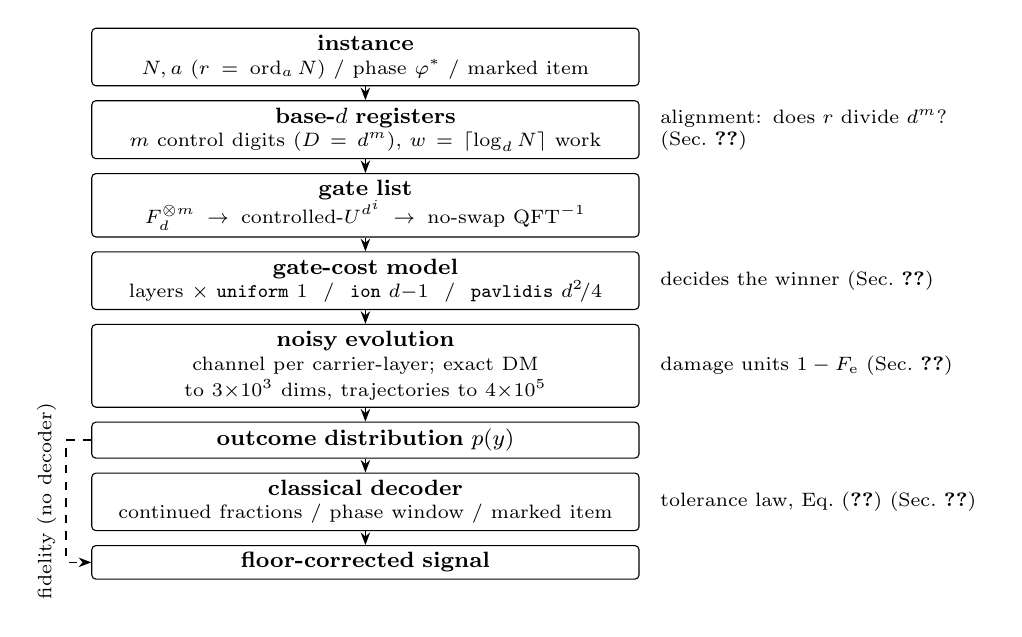
\begin{tikzpicture}[
  font=\footnotesize,
  box/.style={draw, rounded corners=1.5pt, align=center,
              inner ysep=2.5pt, inner xsep=4pt,
              text width=0.55\columnwidth},
  side/.style={font=\scriptsize, align=left, anchor=west,
               text width=0.34\columnwidth},
  arr/.style={-{Stealth[length=1.6mm]}, semithick},
  node distance=5pt
]
\node[box] (inst) {\textbf{instance}\\[-1pt]
  {\scriptsize $N,a$ ($r=\operatorname{ord}_aN$) / phase
   $\varphi^\ast$ / marked item}};
\node[box, below=of inst] (reg) {\textbf{base-$d$ registers}\\[-1pt]
  {\scriptsize $m$ control digits ($D=d^m$),
   $w=\lceil\log_d N\rceil$ work}};
\node[box, below=of reg] (circ) {\textbf{gate list}\\[-1pt]
  {\scriptsize $F_d^{\otimes m}\to\;$controlled-$U^{d^i}
   \to\;$no-swap QFT$^{-1}$}};
\node[box, below=of circ] (cost) {\textbf{gate-cost model}\\[-1pt]
  {\scriptsize layers $\times$ \texttt{uniform} $1$ ~/~
   \texttt{ion} $d{-}1$ ~/~ \texttt{pavlidis} $d^2\!/4$}};
\node[box, below=of cost] (noise) {\textbf{noisy evolution}\\[-1pt]
  {\scriptsize channel per carrier-layer; exact DM to
   $3{\times}10^3$ dims, trajectories to $4{\times}10^5$}};
\node[box, below=of noise] (meas) {\textbf{outcome distribution}
  $p(y)$};
\node[box, below=of meas] (dec) {\textbf{classical decoder}\\[-1pt]
  {\scriptsize continued fractions / phase window / marked item}};
\node[box, below=of dec] (score) {\textbf{floor-corrected signal}};
\draw[arr] (inst) -- (reg);
\draw[arr] (reg) -- (circ);
\draw[arr] (circ) -- (cost);
\draw[arr] (cost) -- (noise);
\draw[arr] (noise) -- (meas);
\draw[arr] (meas) -- (dec);
\draw[arr] (dec) -- (score);
\node[side] at ($(reg.east)+(4pt,0)$)
  {alignment: does $r$ divide $d^m$? (Sec.~\ref{sec:alignment})};
\node[side] at ($(cost.east)+(4pt,0)$)
  {decides the winner (Sec.~\ref{sec:cost})};
\node[side] at ($(noise.east)+(4pt,0)$)
  {damage units $1-\Fe$ (Sec.~\ref{sec:mechanism})};
\node[side] at ($(dec.east)+(4pt,0)$)
  {tolerance law, Eq.~\eqref{eq:decoderlaw}
   (Sec.~\ref{sec:decoder})};
\draw[arr, dashed] (meas.west) -- ++(-9pt,0) |-
  node[pos=0.25, rotate=90, anchor=south, font=\scriptsize]
  {fidelity (no decoder)} (score.west);
\end{tikzpicture}}

\vspace{5pt}

\resizebox{0.96\columnwidth}{!}{%
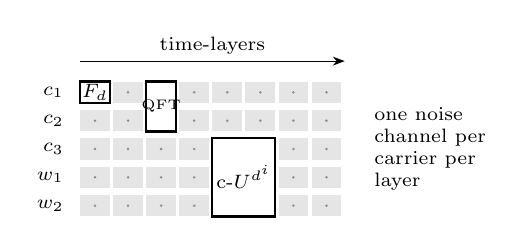
\begin{tikzpicture}[font=\scriptsize, x=0.42cm, y=0.36cm]
\foreach \r/\lab in {0/$c_1$, 1/$c_2$, 2/$c_3$, 3/$w_1$, 4/$w_2$} {
  \node[anchor=east] at (-0.2, -\r) {\lab};
  \foreach \c in {0,...,7} {
    \fill[black!10] (\c, -\r-0.38) rectangle ++(0.9, 0.76);
    \fill[black!45] (\c+0.45, -\r) circle (0.5pt);
  }
}
\draw[thick, fill=white] (0, -0.38) rectangle ++(0.9, 0.76)
  node[midway] {$F_d$};
\draw[thick, fill=white] (2, -1.38) rectangle ++(0.9, 1.76)
  node[midway] {\tiny QFT};
\draw[thick, fill=white] (4, -4.38) rectangle ++(1.9, 2.76)
  node[midway] {c-$U^{d^i}$};
\draw[-{Stealth[length=1.5mm]}] (0, 1.1) -- (8, 1.1)
  node[midway, above=-1pt] {time-layers};
\node[anchor=west, align=left, font=\scriptsize] at (8.6, -2)
  {one noise\\ channel per\\ carrier per\\ layer};
\end{tikzpicture}}
\caption{Top: the simulation pipeline. Every algorithm, base, and
channel flows through the same stages; the four annotations mark where
the paper's main objects enter---the alignment confound at register
choice, the cost model that decides the winner, damage-weighted
exposure in the noise stage, and the decoder whose tolerance obeys
Eq.~\eqref{eq:decoderlaw}. The dashed path is end-state fidelity,
which bypasses the decoder and obeys the one-curve damage law of
Sec.~\ref{sec:mechanism}. Bottom: the exposure convention. Rows are
carriers (control $c_i$, work $w_i$), columns are time-layers; every
carrier passes through the noise channel every layer (dots), a gate
spanning $k$ carriers occupies its cost-model depth in layers (boxes),
and idling carriers decohere while gates execute. Exposure $=$
carriers $\times$ layers; in damage units it is exposure
$\times(1-\Fe)$.}
\label{fig:pipeline}
\end{figure}

\subsection{Algorithms and registers}

We compare three algorithms chosen to span the failure modes of
interference under decoherence. \emph{Shor order finding}: given $N$ and
a coprime $a$, find the multiplicative order $r$ of $a \bmod N$, using a
control register of $m$ base-$d$ digits (control dimension $D=d^m$) and a
work register of $w=\lceil\log_d N\rceil$ digits; success is the
probability that continued-fraction post-processing of the measured
outcome recovers $r$ exactly. Our benchmark instances are unbiased in the
sense of Sec.~\ref{sec:alignment}: $N=21$, $a=2$ ($r=6$) and $N=29$,
$a=16$ ($r=7$). \emph{Eigenstate QPE}: phase estimation on an
eigenstate of a diagonal unitary with target phase equal to the
golden-ratio conjugate $\varphi^\ast\approx0.6180$, chosen to be far
from every fraction with a small base-2, -3, or -5 denominator; success
is the estimate landing within $2^{-(b+1)}$ of the target ($b=5$ bits).
\emph{Grover search} over $M=d^n$ items with
$\lfloor(\pi/4)\sqrt{M}\rceil$ iterations; success is the probability of
measuring the marked item, averaged over a sample of marked items
excluding $\lvert 0\cdots0\rangle$ (the diffuser's own reflection axis
and the bottom of the damping ladder).

Because $M=d^n$ never matches exactly across bases, all cross-base
comparisons are made at matched problem size by interpolating each
base's results onto a common $\log_2$-size axis (linear interpolation
of the signal in $\log_2$ size); comparing raw
demo-size points reverses orderings and is one of the two fairness traps
we document (the other is alignment).

\subsection{Noise channels}
\label{sec:channels}

One time-layer of noise is applied to \emph{every} carrier for every
layer of the serial schedule; a gate spanning $k$ carriers occupies its
decomposition depth in layers (below), so idling carriers decohere while
gates execute.

\emph{Calibrated ladder (transmon-like).} A Lindblad channel with
sequential relaxation $\Gamma_k \propto k^{0.7}$ and pure dephasing
following a max-level law $\Gamma_\phi(j,k)\propto\max(j,k)^{1.1}$,
exponentiated exactly per layer. Both exponents are fits to published
per-level coherence data spanning nine devices and $d=3$ to $12$: the
relaxation ratio $\Gamma_2/\Gamma_1$ is measured at ${\approx}1.7$
\cite{goss2022,blok2021,tripathi2024,peterer2015,yurtalan2020,wang2024}
against $2.0$ for the
textbook $\Gamma_k\propto k$ ladder, and the dephasing ratios
$\Gamma_\phi^{01}:\Gamma_\phi^{12}:\Gamma_\phi^{02}$ are measured at
$1:2.0:2.3$---incompatible with the textbook $(\Delta\mathrm{level})^2$
law (which predicts $1:1:4$) because the charge dispersion of
$\lvert2\rangle$ exceeds that of $\lvert1\rangle$ by an order of
magnitude~\cite{blok2021}. The max-level dephasing target is realized
\emph{exactly} by diagonal jump operators obtained through classical
multidimensional scaling (Sec.~\ref{sec:methods}); our channel
reproduces the measured ratios as $1.62$ and $1:2.14:2.14$. Rates are
normalized so the $0{\leftrightarrow}1$ subspace is bit-for-bit
identical to the qubit channel: every difference between bases is
purely a higher-level effect. A dephasing-scale knob interpolates to the
high-$E_J/E_C$ regime demonstrated at
$d=12$~\cite{wang2024}, where echo coherence approaches the $T_1$
limit; the same knob models refocused operation
(Sec.~\ref{sec:robustness}).

\emph{Per-particle depolarizing (ion-like).} $\rho \to (1-p)\rho + p\,
\mathbb{I}/d$ per carrier-layer. The convention rests on measured
trapped-ion structure: every qudit level is ground-state or metastable
($\tau_1\sim1.1$\,s, orders of magnitude beyond gate times),
allowed-transition magnetic sensitivities span only a factor of
${\sim}5$ (pair dephasing \emph{rates} go as the square, and idling
pairs beyond the driven set widen the span---Sec.~\ref{sec:robustness}
prices the full anisotropy, a $1$--$49\times$ rate spread at $d=5$),
and the single-qudit per-pulse error is nearly flat in $d$
($2.0\times10^{-4}$ at $d=3$, $3.2\times10^{-4}$ at
$d=5$)~\cite{ringbauer2022}, with qudit control demonstrated to 13
levels~\cite{low2023}. A Zeeman-structured dephasing variant that
keeps the encoding's full pair anisotropy is tested in
Sec.~\ref{sec:robustness}.

Measured per-gate noise strengths (rate $\times$ gate time) place
transmon two-qutrit gates at
$7\times10^{-3}$--$3\times10^{-2}$~\cite{goss2022} and ion two-qudit
gates at ${\sim}10^{-3}$~\cite{ringbauer2022,low2023}; our sweeps
($0.001$--$0.05$ at demo size, $0.003$--$0.005$ for scaling) bracket
both operating points, which are marked on every figure.

Four named noise regimes appear in the figures: the \emph{idealized
ladder} ($\Gamma_k\propto k$, $(\Delta\mathrm{level})^2$ dephasing---the
textbook model, used only as a bound), the \emph{calibrated ladder}
above, its \emph{low-charge-dispersion} variant (the dephasing knob set
to the high-$E_J/E_C$ regime of Ref.~\cite{wang2024}), and
\emph{per-particle depolarizing}.

\subsection{Gate-cost models}

Real hardware charges more per entangling gate as $d$ grows, and this is
the strongest objection to any qudit advantage. We charge three
published cost structures as layer multipliers: \texttt{uniform} (native
qudit entangler, one layer regardless of $d$---e.g.\ the cross-Kerr CZ
of Ref.~\cite{goss2022}); \texttt{ion} ($d-1$ per entangling gate,
Ringbauer's $2(d{-}1)$ M{\o}lmer--S{\o}rensen construction normalized to
$1$ at $d=2$---the $d{=}2$ MS gate is itself the two-pulse unit, so
the model charges relative pulse count~\cite{ringbauer2022}); and \texttt{pavlidis} ($d^2/4$ on
all gates, the harshest of the three: the controlled rotations of the
QFT-arithmetic circuits of Ref.~\cite{pavlidis2017} decompose into
$4(d-1)^2$ elementary two-level gates, i.e.\ $(d-1)^2$ per gate after
the same $d=2$ normalization, and our $d^2/4$ charge rounds that cost
\emph{down}---$2.25$ against $4$ at $d=3$, $6.25$ against $16$ at
$d=5$---so the verdicts against decomposed gates below are
conservative). The three
models swing the ququint Shor circuit from $3.8\times$ \emph{shorter}
than the qubit's (15 vs 57 layers on $N=21$) to $1.6\times$
\emph{longer} (93.8 vs 57)---and that swing, not the noise model,
decides the winner. Multi-qudit gates in Grover (oracle and reflection)
are applied as exact unitaries but charged their $n-1$-layer
decomposition depth; charging them one layer would hand the largest free
ride to the base packing the most carriers into the gate, which is
$d=2$. Unless a figure states otherwise, plotted results use the
\texttt{uniform} (native-entangler) cost model---the most
qudit-favorable of the three; Table~\ref{tab:cost} and
Secs.~\ref{sec:cost}, \ref{sec:grover}, and~\ref{sec:robustness}
quantify how the winner changes under \texttt{ion} and
\texttt{pavlidis}.

\subsection{Success metric}

Raw success probabilities have base- and instance-dependent random
floors: a uniformly random outcome passes continued fractions with
probability $0.12$--$0.13$ on the $N=21$ benchmark at demo size,
$0.20$--$0.26$ on $N=29$, and up to $0.59$ on small-order instances.
All comparisons therefore use the floor-corrected signal
\begin{equation}
\mathrm{signal} \;=\;
\frac{\mathrm{success}-\mathrm{floor}}
     {\mathrm{success}_{\mathrm{noiseless}}-\mathrm{floor}},
\end{equation}
which is $1$ for perfect interference, $0$ for random guessing, and
negative when noise actively biases outcomes away from the answer.
Floors and noiseless baselines are recomputed for every base, size, and
readout-error setting. Because small orders compress the metric's
dynamic range, we require a floor-to-baseline span above $0.15$ for
any instance used in a quantitative comparison; the one exception is
the $r=3$ aligned instance of Fig.~\ref{fig:alignment} (spans
$0.07$--$0.12$), retained because no other instance represents its
alignment class---its winner margins far exceed its metric
compression, but we quote no signal magnitudes from it.

% =====================================================================
\section{Grid alignment: a confound that decides winners}
\label{sec:alignment}

Phase estimation concentrates probability on the phases $s/r$. If $r$
divides $D=d^m$, these sit exactly on grid points of the base-$d$
measurement basis and the interference peaks are perfectly sharp;
otherwise they smear over neighboring outcomes, and smeared peaks are
far more fragile under noise. Which base receives sharp peaks is decided
by the arithmetic of the instance, not the physics of the hardware---and
it is invisible in the existing literature because prior studies work at
fixed $d$, where alignment is a constant.

The canonical instance $N=15$ is maximally pathological: its
multiplicative group is $\mathbb{Z}_2\times\mathbb{Z}_4$, so
\emph{every} order is a power of two and the qubit register always lands
exactly on grid while $d=3,5$ never do. Any cross-dimension comparison
run on $N=15$---including the first version of this study---hands base 2
a structural gift unrelated to decoherence.

\begin{figure*}[t]
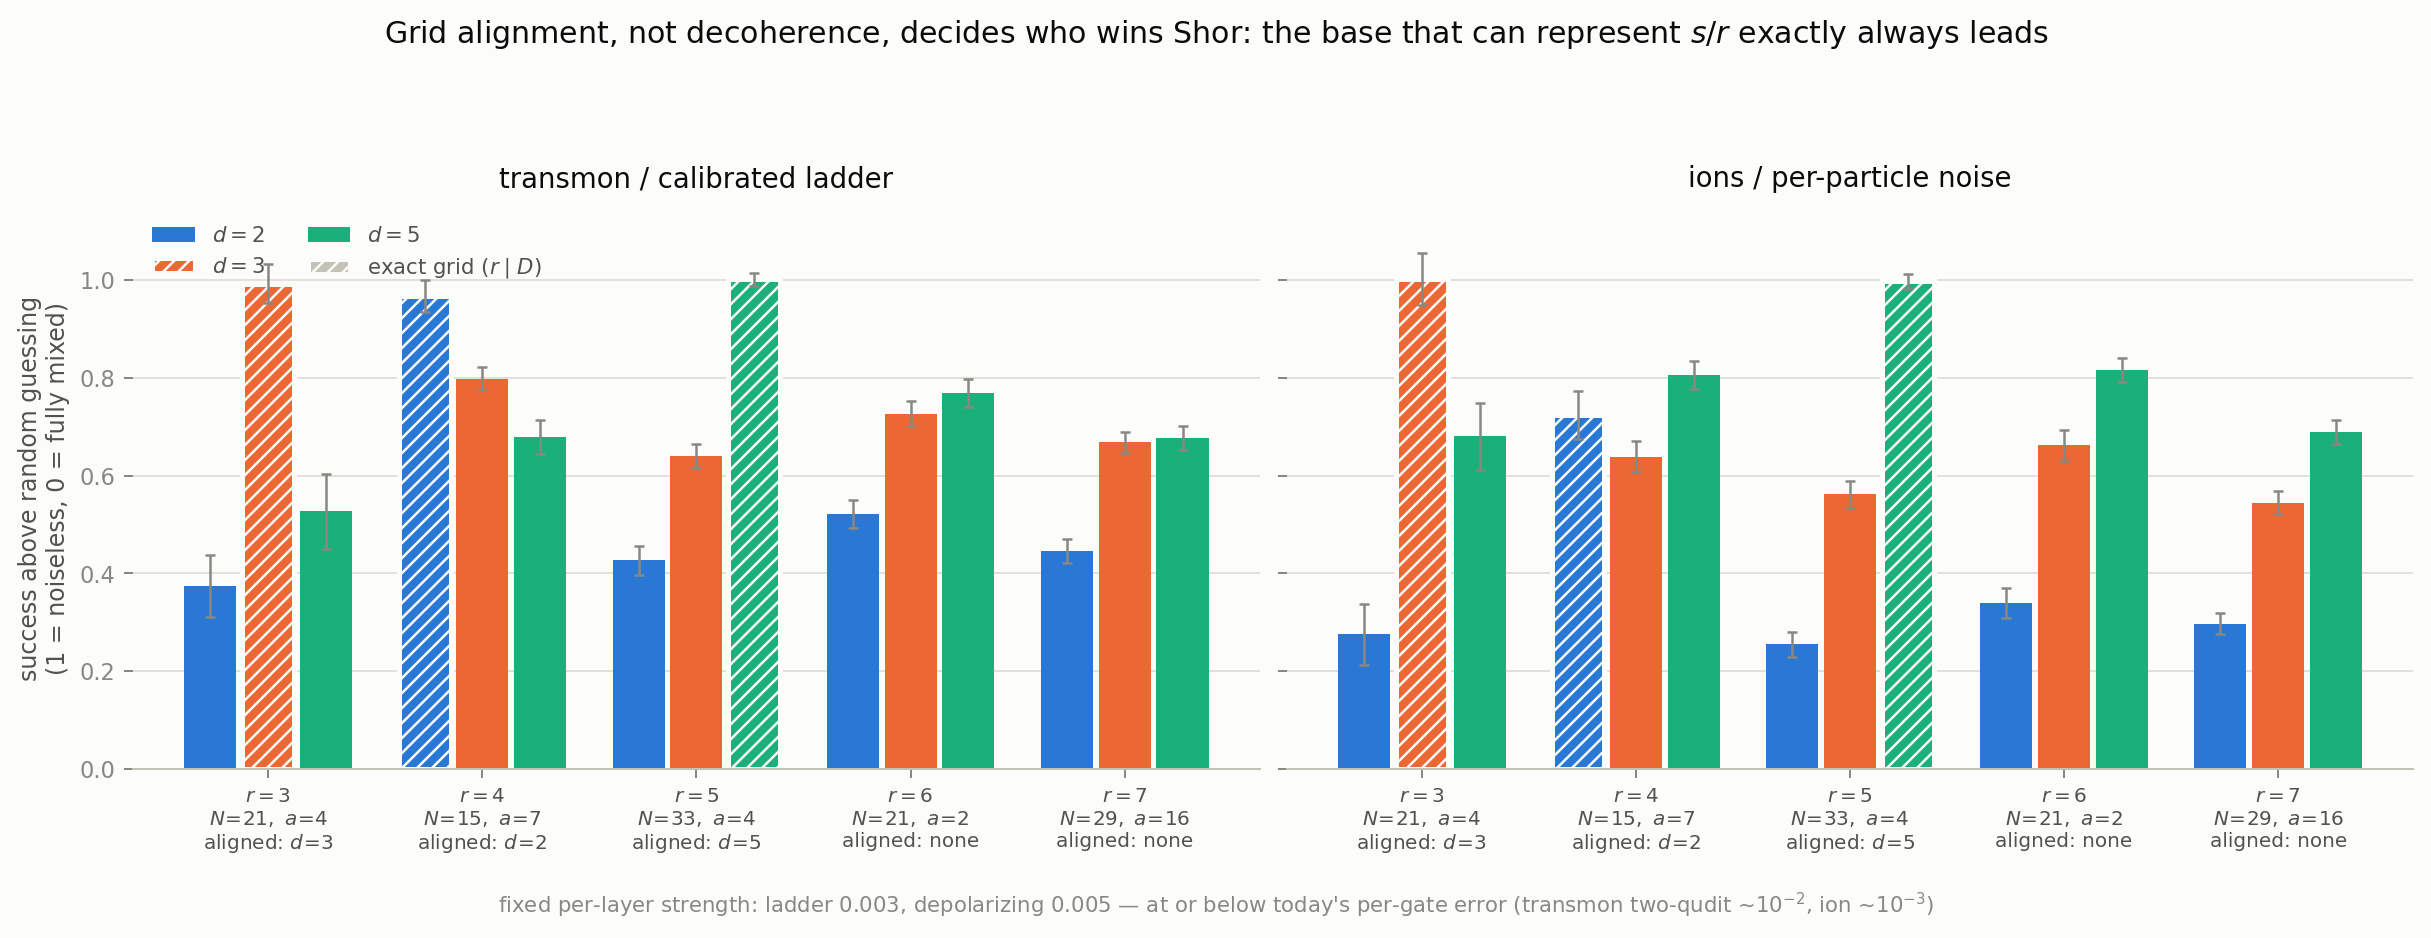
\includegraphics[width=\linewidth]{grid_alignment.png}
\caption{Floor-corrected Shor signal for one instance per alignment
class ($r=3,4,5,6,7$), under calibrated-ladder (strength $0.003$) and
per-particle (strength $0.005$) noise, \texttt{uniform} cost model. The base for which $r$ divides
$d^m$ wins in all six biased runs (three aligned instances $\times$ two
noise models); on both unbiased instances the ordering is
$d{=}5>d{=}3>d{=}2$.}
\label{fig:alignment}
\end{figure*}

Figure~\ref{fig:alignment} shows one instance per alignment class. The
aligned base wins in \textbf{six of six} biased runs, with margins
exceeding anything decoherence produces between bases (at $r=5$ the
aligned ququint scores $1.00$ against the qubit's $0.23$--$0.41$). On
the two unbiased instances ($r=6$, $r=7$) all four runs give the strict
ordering $d=5>d=3>d=2$. Misalignment is moreover graded, not binary:
averaging the distance of the phases $s/r$ to the nearest grid point,
the $r=6$ instance is mildly tilted \emph{toward} the qubit ($0.267$ vs
$0.300$) and the qubit still loses by $0.19$--$0.45$, while $r=7$
($N=29$) is exactly neutral across all three bases---the cleanest
instance we know of, and the one we recommend for future benchmarks.

\emph{Within-modulus control.} Varying $N$ also varies register widths,
so we isolate alignment with two moduli that each host an aligned and an
unaligned order on \emph{identical} registers: $N=33$ and $N=55$ carry
both $r=5$ (exact in base 5) and $r=10$ (exact in no base) with the same
$(m,w)$, gate counts, and noise exposure per base. Removing alignment
costs the ququint $0.14$--$0.22$ signal and narrows its lead over the
qubit by $0.20$--$0.26$, consistently across both moduli and both noise
models---while the ququint's \emph{residual} lead on the unaligned
orders remains $0.38$--$0.57$, twice the alignment term. Both effects
are real; alignment is worth ${\approx}0.2$ signal to whoever receives
it, and the remaining qudit lead is physical. (A converse base-2 control
is impossible to construct: at every modulus large enough to carry both
$r=4$ and a non-power-of-two order, the $r=4$ continued-fraction floor
exceeds its noiseless baseline, collapsing the metric---$N=15$ is the
\emph{only} qubit-aligned instance with usable dynamic range, which is
worth knowing in itself. A consequence is that the ${\approx}0.2$
alignment price is measured only in the ququint-aligned direction and
has no converse check.)

\emph{Ensemble over the multiplicative group.} Shor draws $a$
uniformly from the units of $\mathbb{Z}_N$, so we also score the full
ensemble at $N=21$: all $a\neq1$ in $\mathbb{Z}_{21}^{\times}$
(eleven values; orders $r=6,3,2$ with multiplicity $6,2,3$), exact
density-matrix evolution, \texttt{uniform} cost, both marked
operating points, on the demo registers $D=64/81/125$. Every $r=2$
and $r=3$ instance falls below the $0.15$ span rule of
Sec.~\ref{sec:setup} in every base---small orders collapse the
metric, as disclosed there---so the scorable ensemble is precisely
the unbiased $r=6$ class, where the ensemble-mean signal preserves
the qudit ordering: $0.52/0.73/0.76$ for $d=2/3/5$ on the calibrated
ladder and $0.33/0.67/0.79$ under depolarizing. Raw success needs no
span but carries base-dependent floors ($0.38/0.36/0.39$ on average
here): subtracting them, the full-ensemble excess is
$-0.006/{+}0.030/{+}0.019$ (ladder) and $-0.006/{+}0.028/{+}0.025$
(depolarizing)---so the ensemble-robust statement is that both
qudits clear the qubit, while the $d{=}5>d{=}3$ ordering is a
property of the scorable class rather than of the full ensemble. The ensemble a
Shor user actually samples thus reproduces the fixed-instance
conclusions. The same test at $N=33$ (all $a\neq1$, nineteen values;
orders $r=10,5,2$ with multiplicity $12,4,3$; 400 trajectories per
point)
adds alignment gifts in both directions and closes the loop
quantitatively. The $r=2$ class---base-2 aligned---is unscorable in
every base, floors meeting or exceeding baselines, the converse
collapse documented above; the scorable ensemble splits into the
base-5-aligned $r=5$ class, where the ququint scores $1.00$/$0.97$
(ladder/depolarizing), and the unbiased $r=10$ class, where the
ordering $d{=}5>d{=}3>d{=}2$ holds without any gift ($0.82/0.60/0.45$
and $0.78/0.51/0.23$). The ququint's aligned-over-unaligned excess,
$+0.19$/$+0.18$, independently reproduces the ${\approx}0.2$
alignment price measured by the within-modulus control: the ensemble
structure is predicted class by class. At $N=55$ (all $a\neq1$,
thirty-nine values; adds the base-2-aligned $r=4$ class and $r=20$)
the scorable pattern replicates---the ququint scores $1.00$/$0.99$ on
its aligned class, the unbiased $r=10$ ordering is $0.82/0.58/0.44$
and $0.81/0.49/0.23$, the aligned excess is again $+0.18$, and every
base-2-aligned class ($r=2,4$) is unscorable, the converse collapse
now observed at all three moduli. The modal class, $r=20$ (sixteen of
the thirty-nine), is unscorable in \emph{every} base, and for $d=2$
maximally so: at $D=64$ the noiseless baseline is exactly zero---the
$r=20$ acceptance window contains no outcome at all---the decoder law
of Sec.~\ref{sec:decoder} deciding scorability before noise enters.

\begin{figure*}[t]
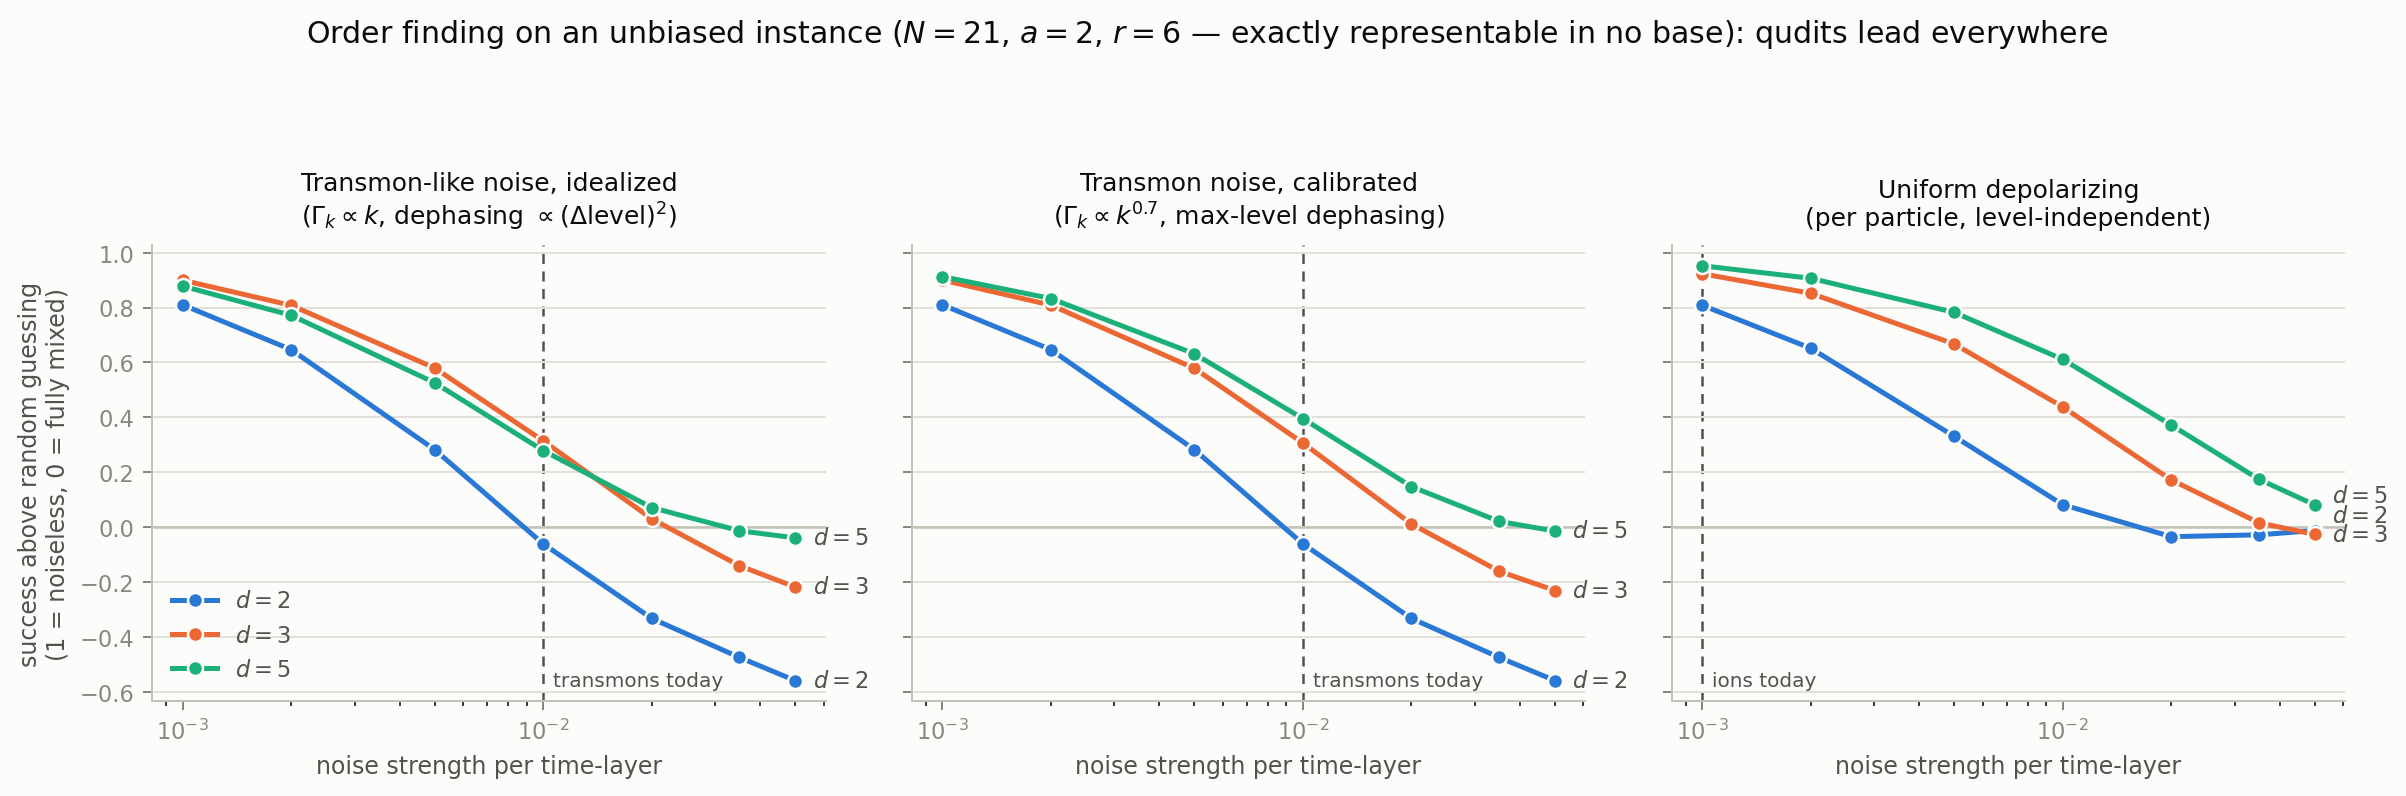
\includegraphics[width=\linewidth]{fair_demo.png}
\caption{Unbiased-instance noise sweep ($N=21$, $a=2$, $r=6$), exact
density-matrix evolution, \texttt{uniform} cost model (native
entangler). Floor-corrected signal vs noise strength for the idealized
ladder, calibrated ladder, and per-particle depolarizing channels. The
best qudit leads the qubit at every strength under all three models;
the single exception to a uniform qudit lead is the deepest
depolarizing point ($s=0.05$), where the qutrit alone dips marginally
below the qubit with all signals within $0.08$ of zero.}
\label{fig:fairdemo}
\end{figure*}

Re-running the full noise sweep on the unbiased instance
(Fig.~\ref{fig:fairdemo}) reverses the study's original conclusion:
the best qudit beats the qubit at every noise strength under \emph{all
three} noise models---including the idealized ladder
($\Gamma_k\propto k$, $(\Delta\mathrm{level})^2$ dephasing), the
harshest treatment of high levels we ever used, under which the qubit
now trails by $0.09$--$0.52$. The earlier ``qubits win Shor on
transmons'' finding was not a noise result at all; it was an
arithmetic artifact, and it does not survive de-confounding under any
model.

% =====================================================================
\section{The cost condition}
\label{sec:cost}

\begin{table}[t]
\caption{Floor-corrected signal on the unbiased instance ($N=21$,
$r=6$) under three gate-cost models, at a single common strength of
$0.005$ for both channels (the middle of the sweep; ladder figures
elsewhere use the marked transmon operating point $0.003$). Rightmost
column: total circuit cost in time-layers for $d=2/3/5$. The winner is
decided by the cost model, not the noise model.}
\label{tab:cost}
\begin{ruledtabular}
\begin{tabular}{llcccc}
noise & cost & $d{=}2$ & $d{=}3$ & $d{=}5$ & layers \\
\hline
depol. & \texttt{uniform}  & 0.331 & 0.667 & \textbf{0.782} & 57/26/15 \\
       & \texttt{ion}      & 0.331 & 0.497 & \textbf{0.502} & 57/44/42 \\
       & \texttt{pavlidis} & 0.331 & \textbf{0.394} & 0.215 & 57/58.5/93.8 \\
ladder & \texttt{uniform}  & 0.282 & 0.578 & \textbf{0.631} & 57/26/15 \\
       & \texttt{ion}      & 0.282 & \textbf{0.374} & 0.256 & 57/44/42 \\
       & \texttt{pavlidis} & \textbf{0.282} & 0.255 & 0.039 & 57/58.5/93.8 \\
\end{tabular}
\end{ruledtabular}
\end{table}

Table~\ref{tab:cost} is the paper's central result in one table. One
direction of the condition holds with a single, instructive
exception: under $d^2$ decomposition (\texttt{pavlidis}) qubits win
in every algorithm, dimension, and channel tested \emph{except} Shor
at $d=3$ under per-particle noise ($0.394$ vs $0.331$ in
Table~\ref{tab:cost}, replicated at 1000-trajectory statistics in the
$d=7$ demo grid, $0.378$ vs $0.312$). The exception isolates the width component of the
mechanism: at $d=3$ the \texttt{pavlidis} depth surcharge almost
exactly cancels the depth compression ($58.5$ vs $57$ layers), while
the width compression (7 vs 11 carriers) survives, and per-particle
damage is nearly flat in $d$---so width alone carries a residual
advantage that the ladder channel, whose per-event damage doubles at
$d=3$, erases. Everywhere else in the grid---the ladder column, the
$d=5$ rows, eigenstate QPE (a dead heat, $0.396$ vs $0.395$), and
Grover in both channels---decomposition forfeits the advantage. Under a native qudit gate
(\texttt{uniform}) the width-and-depth compression is untouched and
qudits win on both hardware classes. The intermediate linear cost
(\texttt{ion}) is where dephasing level decides: on per-particle
hardware the ququint advantage survives ($0.502$ vs $0.331$), while at
free-evolution ladder dephasing the verdict splits---the qutrit still
wins Shor but the ququint loses ($0.256$ vs $0.282$), eigenstate QPE is
a dead heat (advantage $+0.00$), and Grover passes to the qubit for
both qudits (Sec.~\ref{sec:grover}). Refocusing repairs this entire
column (Sec.~\ref{sec:robustness}). Eigenstate QPE (never confounded,
its golden-ratio target phase being irrational in every base) otherwise
tracks Shor, with advantages of $+0.42$ (\texttt{uniform}) and $+0.20$
(\texttt{ion}) on per-particle noise---so the decomposition direction
holds for three genuinely different algorithms, while the converse is
conditional on the dephasing level exactly as the central condition
states.

Cost model and noise model are not independent: each pairing describes a
platform, and both \emph{physically matched} pairings favor
ququints---trapped-ion qudits (\texttt{ion} cost, per-particle noise)
and native-cross-Kerr transmons (\texttt{uniform} cost, calibrated
ladder). The ion pairing presumes shielded, refocused operation;
Sec.~\ref{sec:robustness} prices the unmitigated alternative, and it
is severe. The pessimistic cells of the grid are mostly mismatched
combinations; the genuine failure mode is the absence of a native
entangler (\texttt{pavlidis}), which is precisely the regime of
synthesis-based compilation~\cite{gustafson2025synthesis,venturelli2025}.

\emph{Matched control dimension.} The demo grid compares
$D=64/81/125$, and Sec.~\ref{sec:decoder} shows decoder tolerance
grows with $D$---the ququint enters Table~\ref{tab:cost} with twice
the qubit's acceptance set ($16$ vs $8$ outcomes). Equalizing $D$
resolves the worry in the qudits' favor: at $d=2$, $m=7$ ($D=128$,
matching the ququint's $125$) the qubit scores $0.47/0.30$
(ladder/depolarizing) against $0.51/0.33$ at $D=64$---its extra
decoder tolerance is outweighed by the deeper circuit's added
exposure---while the ququint holds $0.76/0.78$ and the qutrit is
stable between $D=81$ and $243$ ($0.73/0.67$ vs $0.71/0.66$).
Unequal $D$ biases the demo grid against the qudits, not for them.

An independent check: Jankovi\'c \emph{et al.}~\cite{jankovic2023}
derive, by linear response over Haar-random gates under pure dephasing,
the critical gate-efficiency ratio $(d^2-1)/(3\log_2 d)$ a qudit must
clear to beat a qubit register---$1.68$ at $d=3$, $3.45$ at $d=5$, and
$5.70$ at $d=7$, far below the $O(d^2/\log_2 d)$ folklore. Reading our
layer-count ratios as gate-efficiency ratios, their gate-level
criterion predicts our algorithm-level winner in seven of nine
cost/dimension cases on the ladder channel, including the tight case
($d=5$ \texttt{uniform} clears $3.45$ at $3.80$ and wins). Both misses
($d=3$ \texttt{ion}, and $d=7$ \texttt{uniform} below) are in the
conservative direction their pure-dephasing assumption predicts, our
calibrated relaxation being gentler ($\Gamma_k\propto k^{0.7}$).

\emph{The seventh dimension.} A demo-size $d=7$ run on the unbiased
instance (1000 trajectories per point, both channels, all three cost
models; base 7 has the same mean residual misalignment, $0.300$, as
bases 3 and 5) extends the grid one prime higher and sharpens the
condition. The decomposition direction is unchanged: \texttt{pavlidis}
sits at or below the random floor ($-0.05$ to $+0.04$ signal). The
native-gate direction survives---under \texttt{uniform} cost the $d=7$
register beats the qubit on both channels ($0.53$ vs $0.27$ on the
calibrated ladder, $0.80$ vs $0.31$ under depolarizing, at
$s=0.005$)---but on the ladder the ordering is no longer monotone in
$d$: the optimum sits at $d=5$ ($0.65$), the larger per-event damage
of the seventh level pulling $d=7$ back to $0.53$, while under
depolarizing $d=7$ still leads all bases. The intermediate
\texttt{ion} cost, already split at $d=5$, now fails cleanly on the
ladder ($0.07$ vs $0.30$) and retains only a $+0.07$ edge under
depolarizing: the window between native and decomposed cost narrows
with every added level, exactly as the rising break-even curve
suggests. The criterion itself is conservative here---its $d=7$ bar of
$5.70$ is not cleared (the uniform layer ratio is $3.80$), yet the
$d=7$ register wins.

% =====================================================================
\section{Scaling with problem size}
\label{sec:scaling}

\begin{figure*}[t]
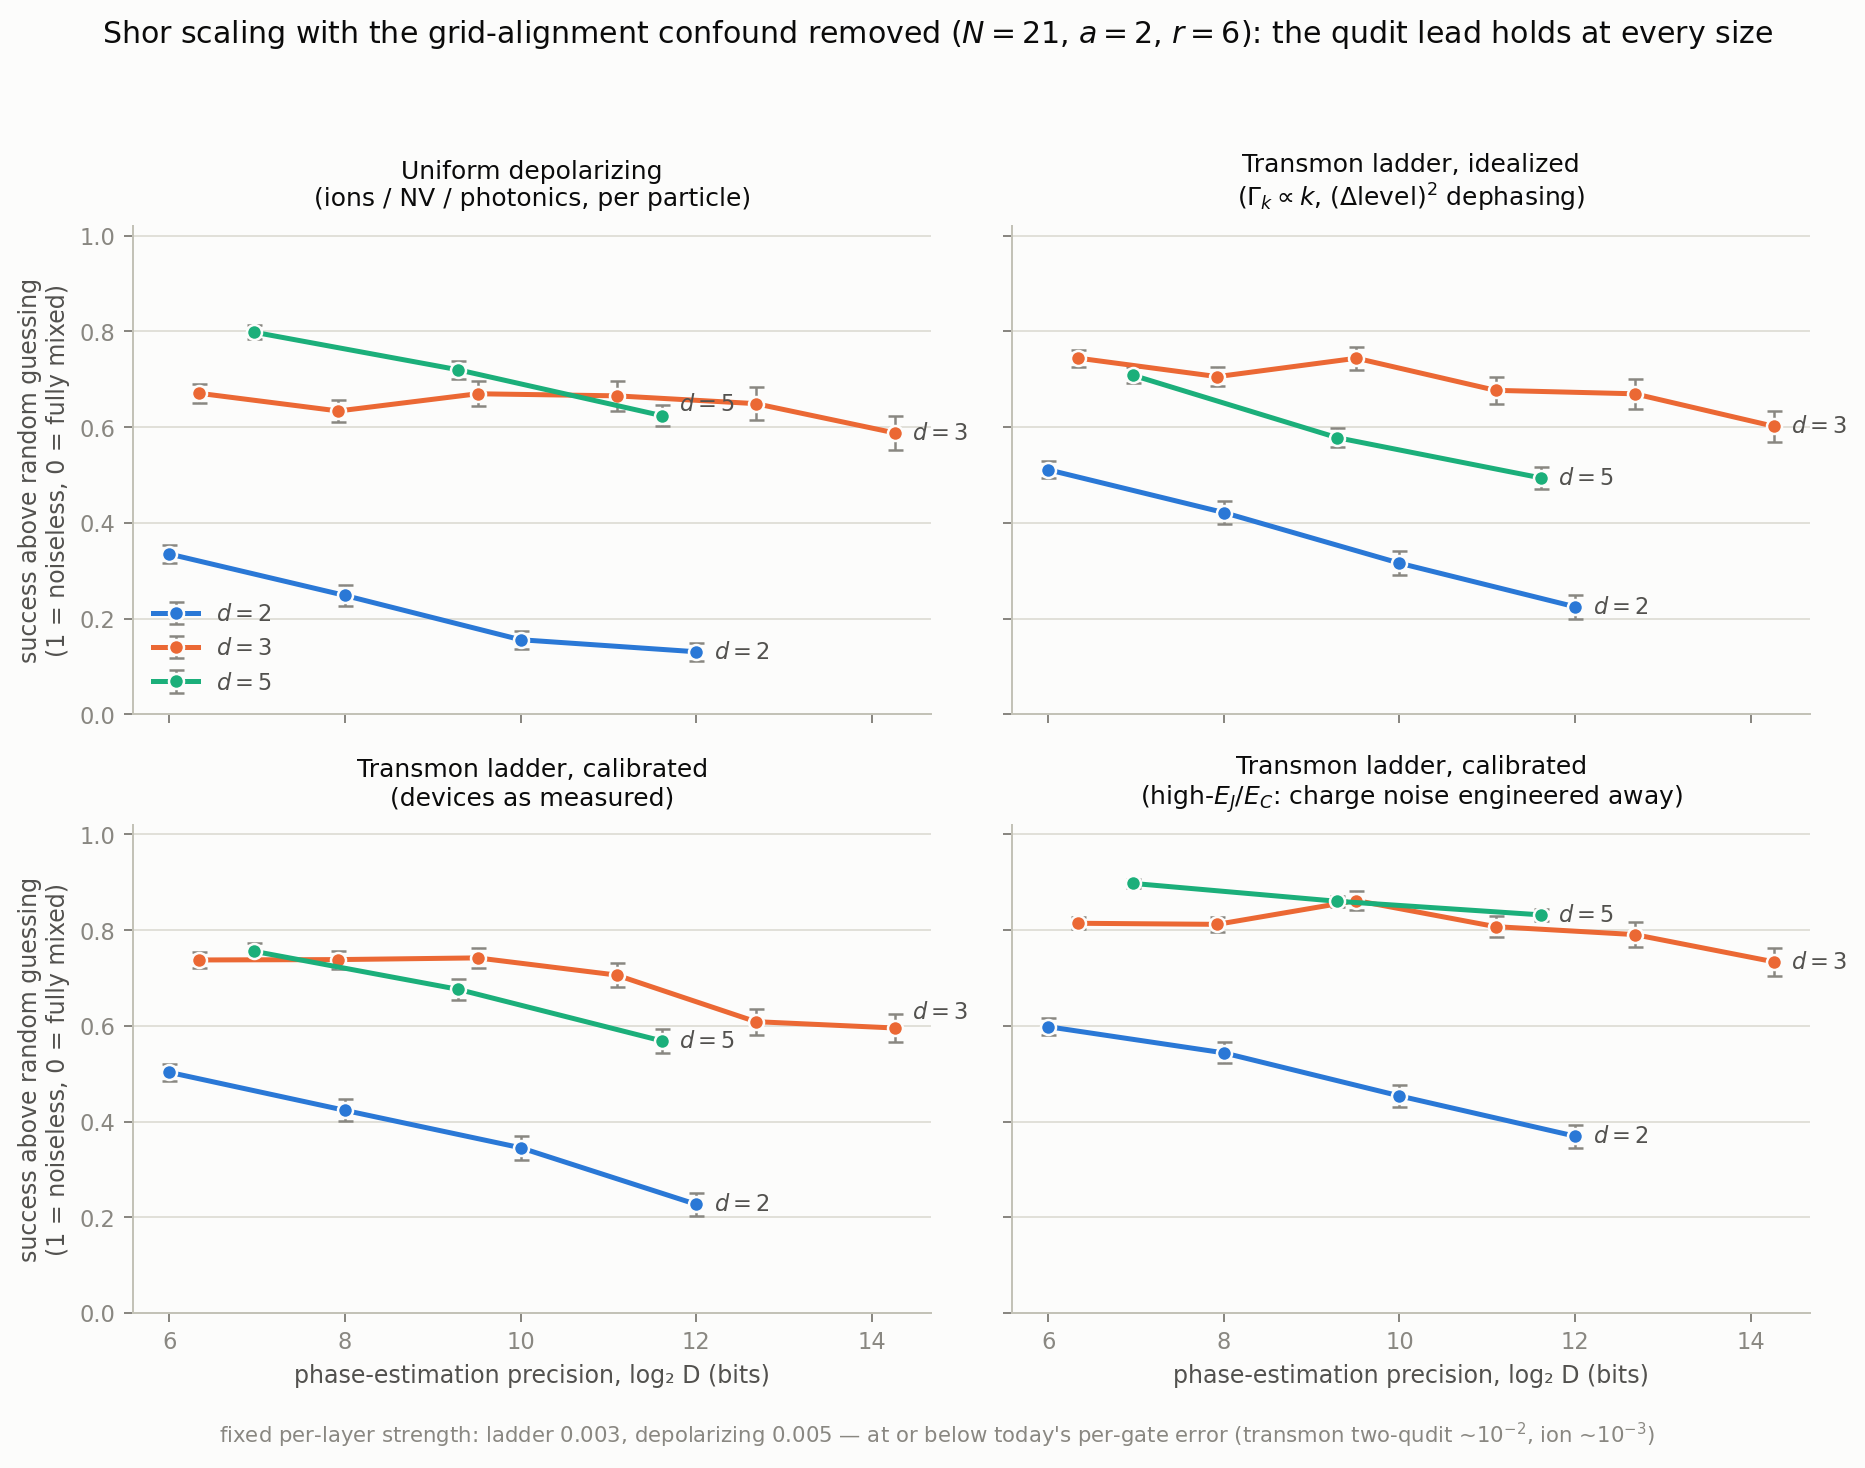
\includegraphics[width=\linewidth]{scaling_fair.png}
\caption{Register-size scaling on the unbiased instance: floor-corrected
signal vs phase-estimation precision (bits), four noise regimes (ladder
regimes at strength $0.003$, depolarizing at $0.005$), \texttt{uniform}
cost model, registers to $5.3\times10^{5}$ Hilbert dimensions, quantum
trajectories (1000 per point).}
\label{fig:scaling}
\end{figure*}

Figure~\ref{fig:scaling} sweeps precision from 6 to 14.3 bits (control
dimensions $64$ to $19683$; the largest register is the qutrit's sixth
size, $m=9$, at $5.3\times10^{5}$ Hilbert dimensions) at fixed
per-layer strength. Both qudits stay above the
qubit at every precision on the measured overlap in all four regimes,
and the gap over the qutrit widens with size under ladder noise
because the qubit decays roughly $2\times$ faster per precision bit:
slopes $-0.045\pm0.003$/bit ($d{=}2$, $R^2=0.99$, $n=4$ sizes) against
$-0.021\pm0.005$/bit ($d{=}3$, $R^2=0.80$, $n=6$) under the calibrated
ladder, while the ququint decays at a rate comparable to the qubit's
($-0.040\pm0.004$/bit, $R^2=0.99$, $n=3$) from a higher starting
point. Two readings deserve emphasis. First, the qutrit's size
dependence is the shallowest in every regime, but it is flat in none of
them: the family holds a plateau and then falls, and a single slope is
therefore a summary rather than a model. Under the calibrated ladder the
first three sizes agree to $\chi^2/\mathrm{dof}=0.01$ ($0.738$--$0.742$
from 6.3 to 9.5 bits) and the whole decline is carried by the last
three, the 14.3-bit point sitting $4.1\sigma$ below the 9.5-bit one.
The same shape appears under depolarizing, where four sizes hold near
$0.67$ before falling to $0.59\pm0.04$ at 14.3 bits, a $1.9\sigma$ drop
from 9.5 bits that turns a slope consistent with zero over the first
five sizes into $-0.007\pm0.004$/bit over six. The onset is later and
the fall gentler in the channel whose per-event damage is flatter in
$d$, which is the ordering Sec.~\ref{sec:mechanism} predicts: the
decoder tolerance of Sec.~\ref{sec:decoder} postpones the decay of
decoded success but does not outrun it. We report the plateau as an
observation with a mechanism, not a law: five sizes would have read as
a flat depolarizing family, and it is the sixth that resolves the
shape. One objection must be met first: $D=d^m$ changes across the
sweep, so the plateau could be residual grid misalignment drifting
with $m$---the confound of Sec.~\ref{sec:alignment} returning in a new
form. It is not. Residual misalignment is \emph{exactly constant}
across the entire sweep for all three bases, on both benchmark
instances ($0.267$ for $d=2$ and $0.300$ for $d=3,5$ at $N=21$;
$0.286$ for every base at $N=29$; spread ${<}10^{-13}$ over the
sizes), because $d^m \bmod r$ is periodic in $m$ and the multiset of
phase offsets it induces therefore repeats. Alignment does not vary
with register size here, so it can explain neither a size-dependent
nor a size-independent signal. On the fitted curves the qutrit
overtakes the ququint at 7.2
bits (calibrated ladder) and 11.3 bits (depolarizing), and from the
smallest common size under the idealized ladder---the story is not
monotonic in $d$, and the best base depends on the target precision.
Second, for eigenstate QPE the qudit advantage is decisive and grows
with size: at 11.6 bits the ququint retains $2.8\times$ the qubit's
signal as measured ($+0.44\pm0.02$) and the margin reaches
$+0.50\pm0.02$ ($2.3\times$) in the high-$E_J/E_C$ regime. Quoted
errors are statistical; the dominant uncertainty is systematic---the
spread across channel and cost-model choices documented above. Since
eigenstate QPE is the quantum-chemistry workhorse, this is the result
with the clearest practical consequence.

\emph{Instance robustness.} Re-running the identical Shor sweep on the
second unbiased instance ($N=29$, $a=16$, $r=7$---the exactly
alignment-neutral benchmark of Sec.~\ref{sec:alignment}, whose work
register is one digit wider for $d=3,5$; 400 trajectories per point)
replicates every claim above. Both qudits again clear the
qubit at every size in all four regimes, and the qubit again decays
fastest ($-0.040\pm0.009$/bit under the calibrated ladder, matching
$-0.045\pm0.003$ at $N=21$; the ququint matches at
$-0.038\pm0.001$ vs $-0.040\pm0.004$). The qutrit's slope agrees
between the instances in both channels---within $0.6\sigma$ under the
calibrated ladder ($-0.025\pm0.004$/bit on $N=29$ against
$-0.021\pm0.005$ at $N=21$) and $1.4\sigma$ under depolarizing
($-0.029\pm0.016$ against $-0.007\pm0.004$)---and is the shallowest in
every regime on both. The $N=29$ sweep stops at four qutrit sizes,
however, so it corroborates the slope without reaching the register
depth at which the plateau above gives way. What is instance-robust is the ordering, the
qubit's fastest decay,
and the late qutrit-over-ququint crossing, which recurs near 11 bits
on $N=29$ under the calibrated ladder (7.2 at $N=21$) and moves
beyond the swept range under depolarizing.

% =====================================================================
\section{Grover search: decomposing the mechanism}
\label{sec:grover}

Everything above measures one algorithm family---the interpolation
experiment of Sec.~\ref{sec:mechanism} shows Shor \emph{is} phase
estimation on an eigenstate superposition. Grover search is the second
family, chosen to attack our own weakest claim, with the prediction
registered in advance: \emph{qudits win, by less than in phase
estimation}. The iteration count $\lfloor(\pi/4)\sqrt{M}\rceil$ is
base-independent, so Grover holds the oracle count fixed across bases;
its residual depth compression comes only from the narrower
multi-qudit decompositions, and at matched size its total exposure
compression is roughly half of Shor's ($5.7\times$ vs $10.9\times$
from $d=2$ to $d=5$). This is a partial rather than a clean
separation of width from depth, but it halves the compression while
holding algorithm structure fixed. A null result would have meant the
advantage was depth all along.

\begin{figure*}[t]
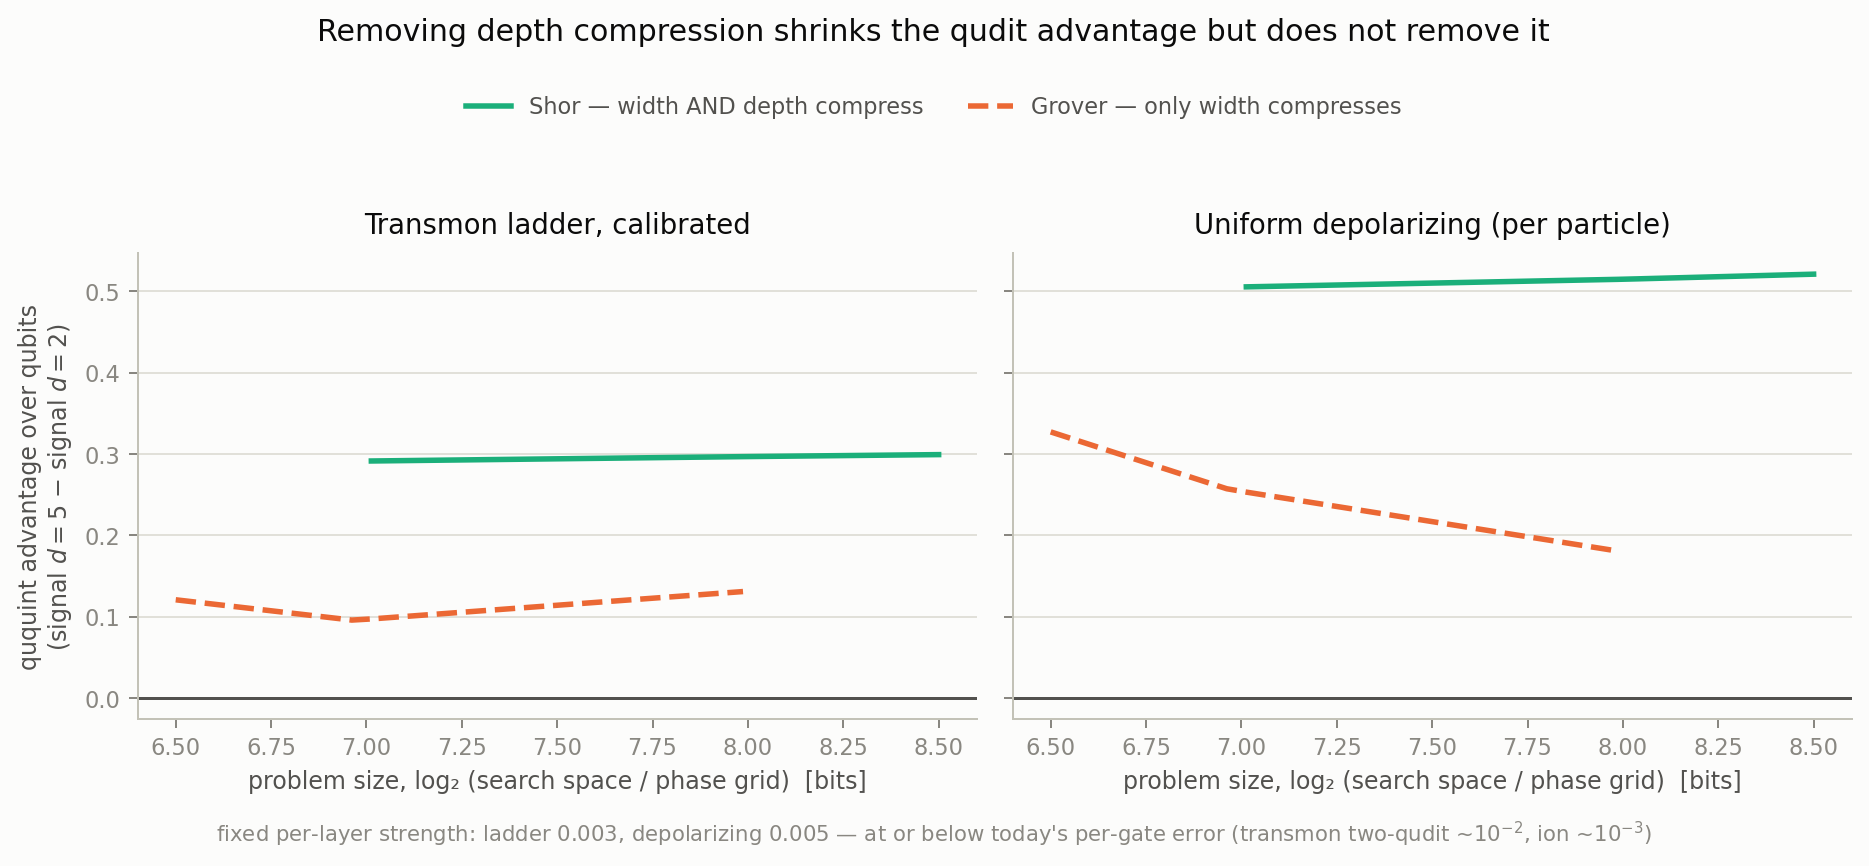
\includegraphics[width=\linewidth]{grover.png}
\caption{Grover vs Shor floor-corrected signal at matched problem size,
both noise models, \texttt{uniform} cost model (native entangler). The
qudit ordering $d{=}5>d{=}3>d{=}2$ holds at every size in both models;
the Grover advantage is $0.33$--$0.50$ of Shor's, consistent with its
halved exposure compression.}
\label{fig:grover}
\end{figure*}

The prediction holds (Fig.~\ref{fig:grover}): the ordering
$d=5>d=3>d=2$ at every matched size in both noise models, with the
Grover advantage at $0.33$--$0.50$ of Shor's. Halving the exposure
compression thus costs one-half to two-thirds of the advantage: the
compressed register is sufficient for a qudit advantage, and the
advantage responds at least proportionally to compression. Grover also
serves as an independent methodological control: it has no order, no
continued fractions, and an exact $1/M$ floor, so grid alignment is
structurally impossible---its agreement rules out the
continued-fraction metric as the source of the effect. The cost
condition binds more tightly here than for Shor: qudits win under
\texttt{uniform} and lose under \texttt{pavlidis} in both channels, and
under \texttt{ion} cost at free-evolution ladder dephasing the
ququint loses Grover at every matched size and the qutrit above
${\approx}6.5$ bits (below which it retains a ${\sim}3\sigma$ edge)
while the qutrit still wins Shor---the cell
where the three algorithms part ways, consistent with Grover's halved
compression buying less headroom against the same gate surcharge, and
the cell that refocusing repairs (Sec.~\ref{sec:robustness}).

% =====================================================================
\section{The mechanism: damage units and the decoder}
\label{sec:mechanism}

\subsection{Entanglement: a falsified hypothesis}

Shor entangles control and work registers; eigenstate QPE does not. An
early hypothesis attributed the (confounded) Shor/QPE difference to
which-path dephasing through the work register. Because Shor's work
input $\lvert x{=}1\rangle$ is an equal superposition of the $r$
eigenstates of the modular multiplier, QPE on a $K$-fold eigenstate
superposition interpolates continuously from eigenstate QPE ($K=1$) to
the Shor regime ($K=r$) with circuit, metric, noise, and cost held
fixed; the control--work entanglement entropy is exactly $\log_2 K$
bits. The measured effect is real but an order of magnitude too small:
${\approx}-0.025$ signal per bit, in all four noise/cost conditions,
against the ${\approx}0.5$ gap---measured on the then-current,
confounded $N=15$ comparison---it was meant to explain (that gap
itself did not survive the de-confounding of
Sec.~\ref{sec:alignment}). We report it as a
falsified mechanism---and it was chasing this failure that exposed the
grid-alignment confound of Sec.~\ref{sec:alignment}.

\subsection{Exposure in damage units, and the decoder boundary}

The surviving mechanism candidate is total noise exposure: carriers
$\times$ time-layers. If it were sufficient, signal would be a function
of exposure $\times$ strength alone and all points---both algorithms,
all bases, all sizes---would collapse onto one curve. They do not
($R^2=0.67$/$0.79$ for ladder/depolarizing), and the failure decomposes
into two identifiable pieces.

\emph{Piece 1: exposure must be counted in damage, not events.} One
noise layer does $d$-dependent harm. Writing $S$ for the one-layer
superoperator, the per-carrier-layer entanglement infidelity is
$1-\Fe$ with $\Fe=\mathrm{tr}\,S/d^2$: under the calibrated ladder at
strength $s$ it is $0.75s$, $1.46s$, and $2.82s$ for $d=2,3,5$---a
ququint takes ${\sim}4\times$ a qubit's damage per event---and
$p(1-1/d^2)$ under depolarizing. With the abscissa
$\mathrm{exposure}\times(1-\Fe)$, Grover's three bases collapse onto a
single exponential: per-family decay rates $0.44/0.49/0.43$ (a $1.1\times$
spread, against $3.6\times$ in event units), each family log-linear with
$R^2\ge0.996$. The reweighting is a ladder effect: depolarizing
damage is already nearly flat in $d$ ($0.75p$--$0.96p$), and there
the signal rows of Table~\ref{tab:collapse} gain nothing from it.

\emph{Piece 2: the residual is the decoder, not the noise.} With units
fixed, a nested fit finds one shared amplitude with a per-\emph{algorithm}
decay rate at $R^2=0.93$/$0.94$ (ladder/depolarizing). The split is stark
at the family level: Grover is a textbook exponential in damage, while
Shor's $d=3$ family holds a flat signal of ${\approx}0.73$ while its
exposure triples. A candidate explanation is that Grover's ``decoder'' is the
identity---its signal \emph{is} marked-state survival---whereas Shor's
signal passes through continued-fraction order recovery, whose error
tolerance grows with register size: added digits add exposure but also
add redundancy the decoder exploits.

\begin{table}[t]
\caption{The collapse test: goodness of a single two-parameter
exponential $A e^{-kx}$ pooled over both algorithms, all bases and
sizes.}
\label{tab:collapse}
\begin{ruledtabular}
\begin{tabular}{llcc}
ordinate & abscissa & ladder $R^2$ & depol.\ $R^2$ \\
\hline
signal   & exposure $\times$ strength & 0.67 & 0.79 \\
signal   & exposure $\times$ damage   & 0.81 & 0.79 \\
fidelity & exposure $\times$ damage   & \textbf{0.97} & \textbf{0.99} \\
\end{tabular}
\end{ruledtabular}
\end{table}

This is directly testable: if the decoder story is right, end-state
\emph{fidelity} $\langle\psi_{\mathrm{ideal}}\rvert\rho\lvert
\psi_{\mathrm{ideal}}\rangle$ should obey the one-curve law that signal
does not. It does (Table~\ref{tab:collapse}): one shared exponential in
damage units fits the fidelity of both algorithms at $R^2=0.97$ (ladder)
and $0.99$ (depolarizing), with fitted amplitude ${\approx}1$ as the
zero-noise limit demands; granting the algorithms separate rates adds
only $0.02$/$0.003$. The decoder gap is visible in the raw numbers:
Grover's fidelity equals its signal to better than $0.006$ under the
ladder and $0.025$ under depolarizing at every point, while Shor's
$d=3$ family loses two thirds of its fidelity ($0.55\to0.18$) with
signal flat, and at $d=2$, $m=12$ under depolarizing, continued
fractions decode a signal of $0.093\pm0.025$ from a state with
fidelity $3\times10^{-4}$. The mechanism claim, in the form the data
support: \emph{accumulated channel damage is the law for the quantum
state; the residual algorithm dependence of decoded success sits in
the decoder}---for which Sec.~\ref{sec:decoder} gives an exact
quantitative account, derived and verified against the decoder
itself.

\emph{What the collapse does and does not prove.} For a product of
near-identity incoherent channels, log-fidelity is additive in the
per-application entanglement infidelity to first order, so a single
exponential with amplitude ${\approx}1$ is the \emph{null
expectation}, not a discovery. The informative content of
Table~\ref{tab:collapse} is therefore bounded as well as measured. In
linear fidelity the shared fit gives $R^2=0.97/0.99$; rescored in
\emph{log} fidelity---the metric that weights the deep tail---the
same fit gives $R^2=0.76$ in both channels ($0.85$--$0.91$ if refit
there). The law holds within a factor of two down to fidelity
$1.5\times10^{-2}$ on the ladder and, excepting a single
floor-pinned Grover point, to $2.7\times10^{-4}$ under depolarizing;
every departure is a Grover point approaching its
$1/\!\dim\mathcal{H}$ fidelity floor (the deepest, at
$5.3\times10^{-3}$, sits $1.4\times$ above its floor of $1/256$ and
$82\times$ above the fit)---a floor that varies across exactly the
bases and sizes the collapse unifies. What survives everywhere is
the decoder residual, which no channel-level argument predicts. Conversely, the law's failure mode
is error that does not compose incoherently: correlated or coherent
noise breaks the additivity, and that is precisely what the deep
hardware circuit exhibits (Sec.~\ref{sec:hardware})---which is why
the law is stated for Markovian incoherent channels only (see
Limitations).

\begin{figure*}[t]
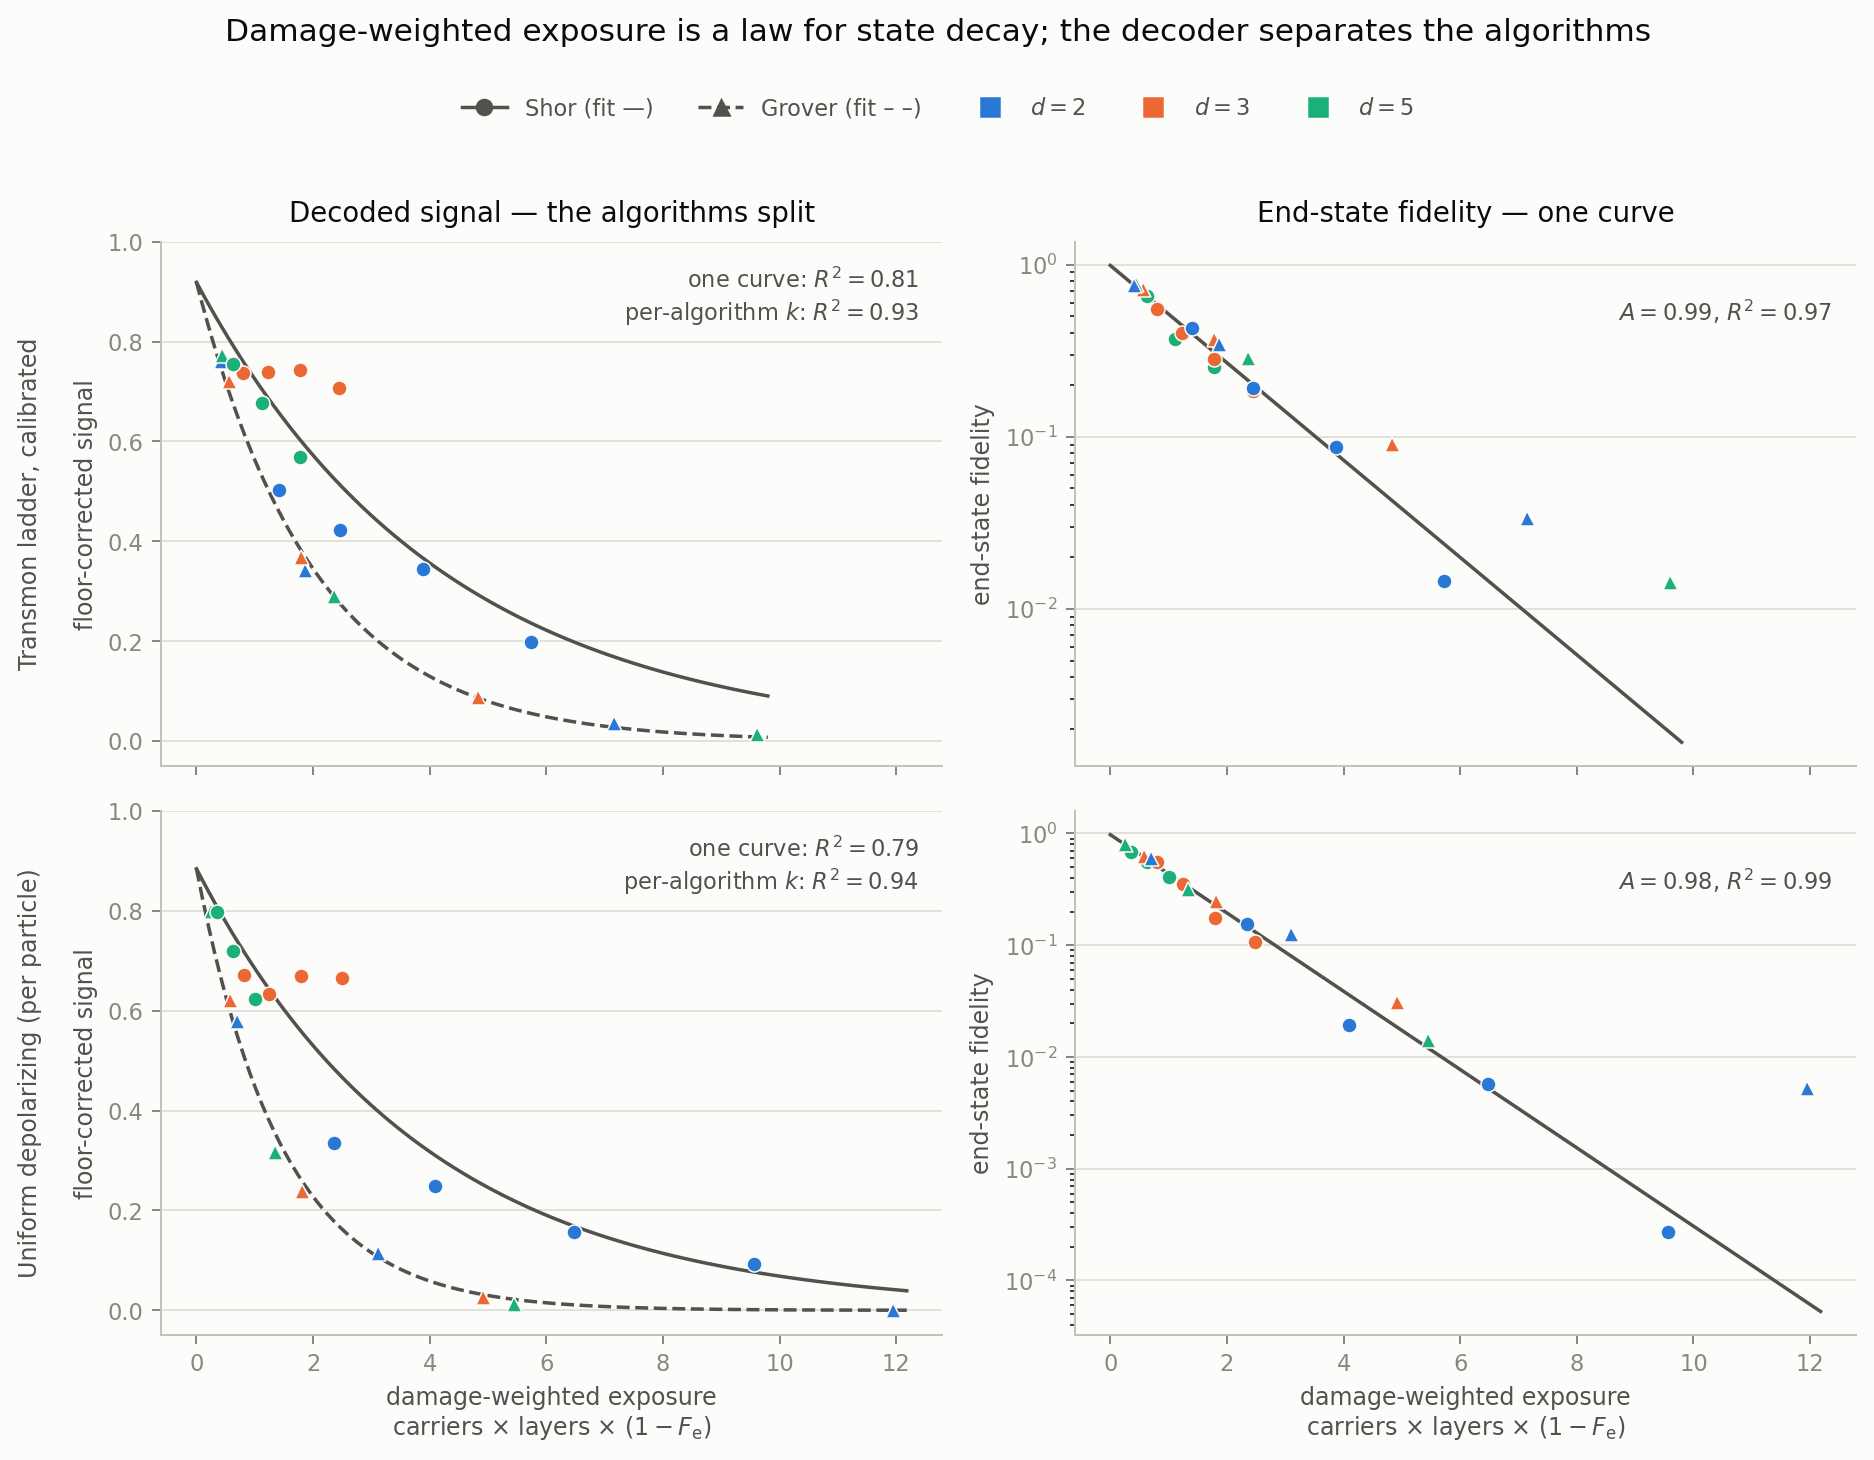
\includegraphics[width=\textwidth]{mechanism.png}
\caption{Damage units and the decoder. Left column: floor-corrected decoded
signal against damage-weighted exposure---the algorithms refuse a common
curve ($R^2=0.79$--$0.81$), and granting a per-algorithm decay rate
(solid: Shor; dashed: Grover) recovers $R^2=0.93$--$0.94$; Shor's $d=3$ family
(orange circles) sits nearly flat while its exposure triples. Right
column: end-state fidelity on the same abscissa (log scale) falls on a
single exponential with amplitude ${\approx}1$ for both algorithms, all
bases and sizes ($R^2=0.97$/$0.99$; \texttt{uniform} cost model). The residual algorithm structure in
decoded signal is therefore the classical decoder, not unexplained noise
physics.}
\label{fig:mechanism}
\end{figure*}

\subsection{Why the decoder gains tolerance with size}
\label{sec:decoder}

The size dependence of Shor's decoder tolerance has a closed form, and
because the decoder is classical we can measure it exactly rather than
argue it. Continued-fraction recovery succeeds for any outcome $y$
whose phase $y/D$ lies within $1/(2r^2)$ of some $s/r$---the classical
convergent guarantee~\cite{hardy2008,shor1997}. This sufficient
condition gives an acceptance window around each of the $r-1$ peaks
spanning $1/r^2$ in phase and holding ${\sim}D/r^2$ outcomes, while the
noiseless interference peak stays ${\sim}1$ outcome wide at every
size. The window therefore grows
linearly in $D=d^m$, exponentially in register size, whereas
noise-induced broadening grows only polynomially in $m$ (exposure $=$
carriers $\times$ layers). The decoder's redundancy therefore outpaces
the added exposure over a range of sizes, which is why Shor's signal
families hold a plateau while their fidelity decays exponentially---and
why Grover, whose acceptance set is the single marked item at every
size, shows no such plateau. The reprieve is finite: the acceptance set
grows linearly in $D$ but the accepted outcomes must still carry
amplitude, and once fidelity has fallen far enough the decoded signal
follows, which is the fall the sixth qutrit size exposes in
Sec.~\ref{sec:scaling}. Decoder tolerance postpones the decay of
decoded success; it does not repeal it.

\begin{table}[t]
\caption{The decoder measured, not estimated: exact size of the
continued-fraction acceptance set $A=\{y\in[0,D): \text{decode}(y)=r\}$
on the benchmark instance ($N=21$, $r=6$), obtained by running the
decoder over every outcome. ``per peak'' is $\lvert A\rvert/(r-1)$;
the envelope estimate is $D/r^2$; ``law'' is the totient sum of
Eq.~\eqref{eq:decoderlaw} per peak, whose exact finite-$D$ form (see
text) reproduces $\lvert A\rvert$ without error at every size. No
simulation is involved.}
\label{tab:decoder}
\begin{ruledtabular}
\begin{tabular}{ccrrrrr}
$d$ & $m$ & $D$ & $\lvert A\rvert$ & per peak & $D/r^2$ & law \\
\hline
2 & 6  & 64   & 8   & 1.6   & 1.8   & 1.8   \\
2 & 8  & 256  & 36  & 7.2   & 7.1   & 7.2   \\
2 & 10 & 1024 & 148 & 29.6  & 28.4  & 28.9  \\
2 & 12 & 4096 & 582 & 116.4 & 113.8 & 115.7 \\
3 & 4  & 81   & 10  & 2.0   & 2.2   & 2.3   \\
3 & 5  & 243  & 36  & 7.2   & 6.8   & 6.9   \\
3 & 6  & 729  & 100 & 20.0  & 20.2  & 20.6  \\
3 & 7  & 2187 & 308 & 61.6  & 60.8  & 61.8  \\
5 & 3  & 125  & 16  & 3.2   & 3.5   & 3.5   \\
5 & 4  & 625  & 88  & 17.6  & 17.4  & 17.6  \\
5 & 5  & 3125 & 442 & 88.4  & 86.8  & 88.2  \\
\end{tabular}
\end{ruledtabular}
\end{table}

Table~\ref{tab:decoder} runs the project's own continued-fraction
routine over every outcome $y\in[0,D)$ and counts the acceptance set
exactly; the growth from $1.6$ accepted outcomes at $D=64$ to $116$ at
$D=4096$ is a $73\times$ gain in tolerance against a peak that never
widens. The acceptance set moreover has an exact description. The
decoder accepts $y$ if and only if some convergent denominator $q$ of
$y/D$ is a multiple of $r$ with $q\le N$ (Appendix~\ref{app:decoder}
proves the equivalence and reconciles it with the divisor-form
recovery of the standard analyses), which reduces $A$ to pure
number theory: for a reduced fraction $p/q$, the phases with $p/q$
among their convergents form the open interval between the
Stern--Brocot mediants $(p+p')/(q+q')$ and $(2p-p')/(2q-q')$, where
$p'/q'$ is the penultimate convergent of $p/q$---a classical fact of
continued-fraction theory~\cite{khinchin1964,hardy2008}. Partitioning outcomes
by the \emph{first} admissible convergent of $y/D$ makes the
decomposition disjoint (the side denominator $q-q'$ is never a
multiple of $r$, since $\gcd(q',q)=1$), and summing the interval
counts reproduces the enumerated $\lvert A\rvert$ \emph{without
error}---outcome for outcome, on all 27 instance/size combinations
tested, including all four within-modulus orders. Summing interval
measures instead of counts gives the asymptotic law
\begin{equation}
\frac{\lvert A\rvert}{D}\;\longrightarrow\;
2\ln 2\sum_{k=1}^{\lfloor N/r\rfloor}\frac{\varphi(kr)}{(kr)^2},
\label{eq:decoderlaw}
\end{equation}
with $\varphi$ Euler's totient (the exact per-denominator measure is
$\mu(q)=\tfrac{2}{q}\sum_{u<q,\,\gcd(u,q)=1}(q+u)^{-1}\to
2\ln2\,\varphi(q)/q^2$; summed over \emph{all} denominators $q\le Q$
this weight reproduces the almost-everywhere count
$(12\ln2/\pi^2)\ln Q$ of convergent denominators below
$Q$~\cite{khinchin1964}, so the measure itself is classical---the
content of Eq.~\eqref{eq:decoderlaw} is its restriction to the
denominators the decoder admits); it holds to better than $1\%$ on five of our
six instances at $D\gg N^2$, and to $4.2\%$ on the sixth ($N=55$, $r=5$,
where eleven admissible denominators make the first-admissible
exclusions largest). The law settles both scaling directions at once.
In $D$ it is exactly linear---the measured $\lvert A\rvert\propto
D^{1.03\pm0.01}$ ($R^2=0.999$) carries its small excess over slope 1
purely from window discreteness. In $r$ it replaces the $1/r^2$
envelope: comparing $r=5$ with $r=10$ on identical registers (the
within-modulus pairs of Sec.~\ref{sec:alignment}, swept to $D\ge5r^2$
so the window exceeds one outcome) gives measured per-peak ratios of
$9.6$ ($N=33$) and $8.9$ ($N=55$) where $1/r^2$ predicts $4.0$; the
law's totient-sum ratios are $9.7$ and $9.3$. It also explains the
envelope's apparent success in Table~\ref{tab:decoder} as an accident
of the benchmark instance: at $r=6$, $N=21$ the naive $(r-1)/r^2=0.139$
sits within $2\%$ of the law's $0.141$ because two errors
compensate---the true $q=r$ window measure $2\ln2\,\varphi(r)/r^2$ is
only $0.55\times$ the envelope's, and the admissible multiples
$2r,\dots,\lfloor N/r\rfloor r$ restore the difference. On the $r=5$
instances, where the cancellation fails, the envelope is off by
$2.5$--$3\times$ while the law stays within $4.2\%$.

\emph{Relation to success-probability analyses of order finding.} An
exact literature bounds the success of continued-fraction
post-processing on base-2 registers: Shor's original $4/\pi^2$
asymptotics~\cite{shor1997}, the sharp divisor-recovery bounds of
Gerjuoy~\cite{gerjuoy2005} and of Bourdon and
Williams~\cite{bourdon2007}, Eker{\aa}'s proof that a single run
recovers $r$ with probability approaching one~\cite{ekera2024}, the
tight two-sided window bounds of Magdon-Ismail and
Dong~\cite{magdon2025}, the self-contained treatise of Barzen and
Leymann~\cite{barzen2022}, and, for eigenstate phase estimation,
Chappell \emph{et al.}~\cite{chappell2011}. These analyses score
outcomes inside a tolerance window of the peaks via the convergent
guarantee---a sufficient condition---and typically certify recovery
of a divisor $r/\gcd(s,r)$ that a classical search then lifts to $r$.
The law above differs in kind: it is an exact, outcome-for-outcome
description of the full acceptance set of a decoder that must return
$r$ itself, including the contribution of the admissible denominators
$2r,\dots,\lfloor N/r\rfloor r$ that window bounds do not count.
Eq.~\eqref{eq:decoderlaw} depends only on $r$ and $N$, not on the
base: at matched control dimension the decoder's tolerance is
\emph{identical} across bases, so the entire cross-base difference in
decoded success sits in the quantum state---precisely this section's
mechanism claim. We are not aware of this acceptance set having been
computed before for a decoder required to return $r$ itself.

This decomposition has a general reading beyond the present comparison.
A decoded success probability conflates two quantities with different
physics: the decay of the quantum state, which damage-weighted exposure
describes universally, and the error tolerance of the classical
post-processing wrapped around the measurement, which is
algorithm-specific and can grow with problem size. Benchmarks of
``noise resilience'' across algorithms or encodings that use decoded
success as their metric are therefore partially measuring decoder
redundancy---a classical resource. Reporting end-state fidelity
alongside decoded signal, as in Table~\ref{tab:collapse}, separates the
two at no extra simulation cost, and we suggest it as standard practice
for noisy-algorithm comparisons.

% =====================================================================
\section{Robustness}
\label{sec:robustness}

\emph{Readout error.} A $d$-level readout must resolve $d$ pointer
states, the higher ones worst. Charging a readout channel with misread
rate of $\lvert k\rangle$ growing as $(1+k)$---a linear reading of the
few-percent, higher-is-worse readout errors reported for transmon
qutrits~\cite{blok2021,goss2022}---on every control carrier of every
base leaves the qudit advantage untouched: the ququint's lead drifts
by less than $\pm0.03$ over the full sweep $\varepsilon=0$--$0.04$ (an
$8\times$ range among nonzero settings). The reason is a structural cancellation: total readout
exposure is $m\times\varepsilon(d{+}1)/2$, and at matched precision
$m\approx\log D/\log d$, giving $9\varepsilon/8\varepsilon/9\varepsilon$
for $d=2/3/5$ at $D\approx64$. Per-level readout degradation with $d$ is
almost exactly cancelled by the reduced carrier count---near-neutral by
construction, not luck. The neutrality claim is scoped to
simultaneous $d$-level discrimination (the transmon case that
motivates the $(1{+}k)$ model): ion-qudit readout is sequential
shelving with $d-1$ detection rounds, so misreads compound down the
sequence and readout \emph{time} grows with $d$, adding idle
decoherence the cancellation above does not include.

\emph{Refocusing.} No transmon runs a long circuit without echo, so the
honest question is whom it helps more. Sweeping the dephasing scale from
free evolution to perfect echo (the same knob that models the
high-$E_J/E_C$ regime~\cite{wang2024}), the ququint's lead grows
monotonically in all four conditions tested. The consequential case is
linear-in-$d$ gate cost: the ququint \emph{loses} Shor without echo
($-0.026$) and \emph{wins} with it ($+0.191$); QPE moves from exact
parity to $+0.196$. Mechanistically, dynamical decoupling suppresses
dephasing---the part of the ladder channel scaling worst with $d$ (the
max-level law)---and leaves the gentler $k^{0.7}$ relaxation, in
agreement with qudit DD experiments~\cite{tripathi2024} and with the
refocused molecular-qudit QFT of Ref.~\cite{rubinosanz2025}. This is why
the central condition is stated ``at the device's operating dephasing
level'': refocusing buys roughly one cost model of headroom, and
benchmarks of qudit algorithms should be run on refocused devices.

\emph{Noise-inflation threshold.} The channels charge every base the
same per-layer strength; if higher-$d$ gates are additionally noisier
per layer, the condition acquires a threshold. Inflating the qudit's
per-layer strength alone, $s_d=f\,s_2$, and locating the crossing
$f^\ast$ at which the qudit's floor-corrected signal falls to the
qubit's (demo instance, exact density matrices, both operating
points): under native-gate cost $f^\ast=2.0$--$2.5$ on the calibrated
ladder and $2.6$ ($d{=}3$) to $4.5$ ($d{=}5$) under depolarizing;
under the linear \texttt{ion} cost $f^\ast=1.2$ ($d{=}3$, ladder) and
$1.6$ ($d{=}3,5$, depolarizing), the ladder ququint cell being
already lost at $f=1$ (Sec.~\ref{sec:cost}). Read as hardware
guidance: a platform keeps the qudit advantage while its measured
qudit-to-qubit per-gate noise ratio stays below $f^\ast$ \emph{after}
the layer-count multiplier is charged---roughly $1.6\times$ for
today's trapped-ion pairing and $2.0$--$2.5\times$ for a
native-entangler transmon (the calibrated-ladder/\texttt{uniform}
pairing; the $4.5\times$ cell belongs to
depolarizing/\texttt{uniform}, a crossed pairing).

\emph{Zeeman-structured dephasing.} The per-particle convention
flattens pair structure the ion encoding really has, so we also test
its worst case: magnetic-field dephasing carrying the collective-$B$
sensitivity structure of the $^{40}$Ca$^{+}$ level indexing of
Ref.~\cite{ringbauer2022}, applied independently per carrier---the
uncorrelated worst case---realized exactly by a single diagonal jump
$\propto\mathrm{diag}(g_j m_j)$ ($g_S=2$, $g_D=6/5$; the Markovian
generator stands in for the unrefocused effect of what is, in the
laboratory, quasi-static noise), normalized so the optical-qubit pair
$0{\leftrightarrow}1$ matches the qubit channel. Pair rates then span
$1$--$25\times$ that reference at $d=3$ and $1$--$49\times$ at $d=5$.
The encoding is no strawman: over all $\binom{8}{d}$ level subsets of
the $S_{1/2}$/$D_{5/2}$ manifold, the chosen levels exactly minimize
the worst pair rate at $d=5$ and $d=7$; only $d=3$ admits a gentler
choice ($9\times$, via $\{S_{-1/2},D_{-3/2},D_{-1/2}\}$). The verdict
reverses outright: the qubit wins at every strength under both cost
models ($0.72$ against $0.24$/$0.23$ at $s=0.003$, \texttt{uniform}).
Nor is the missing correlation structure doing the work: repeating
the study with genuinely common-mode dephasing---one global jump
coupling to the total Zeeman shift, exact as an elementwise mask on
the density matrix---preserves the reversal ($0.87$ against
$0.45$/$0.34$ at the same point; its decoherence-free pairs soften
every base, the qubit most). Unmitigated Zeeman-structured dephasing
on a sensitivity-ordered encoding is therefore a regime with no qudit
advantage at all---the sharpest failure mode we found, and one the
condition's ``operating dephasing level'' clause must be read to
include. Measured devices are engineered away from this regime: shielding
makes coherence times of order $100$\,ms achievable across all
transitions~\cite{ringbauer2022}. The device's randomized
benchmarking---per-pulse error rising only $1.6\times$ from $d=3$ to
$d=5$ ($2.0\times10^{-4}$ to $3.2\times10^{-4}$) where the raw
sensitivity ratio is $25$--$49$---is consistent with a near-flat
residual, though a few-microsecond pulse cannot resolve slow
dephasing; the direct evidence the convention needs is $d$-resolved
Ramsey or echo coherence across the encoding's transitions, and
pending that, the per-particle convention is a statement about
mitigated hardware whose price of failure the following sweep fixes.
The mechanism mirrors the refocusing result above---structured, slow
dephasing is exactly the part echoes remove---and the price is
quantitative: composing the Zeeman component with the depolarizing
operating point ($s=0.005$; the two channels commute, so the product
is exact) and sweeping the suppression factor $\varepsilon$ applied
to the unmitigated Zeeman reference ($s_Z=0.003$ per carrier-layer),
the qudit ordering returns at $\varepsilon^\ast=0.58$--$0.79$ under
native-gate cost but only at $\varepsilon^\ast=0.09$--$0.15$ under
the $2(d{-}1)$ M{\o}lmer--S{\o}rensen cost. In hardware units the bar
is a $0{\leftrightarrow}1$-pair coherence of ${\gtrsim}400$--$600$
layer times for native-gate cost and ${\gtrsim}2200$--$3800$ for MS
cost: at ${\sim}100\,\mu$s layers, a $100$\,ms shielded coherence
meets the native-gate bar with a factor-two margin but falls short
of the MS-cost bar by $2$--$4\times$. On linear-cost hardware the
Zeeman component must be suppressed below the plain shielding
level---deeper echo sequences or magnetically insensitive
encodings---before the qudit ordering returns.

\emph{Composite dimension.} Nothing in the circuits or channels uses
primality. A $d=4$ point on the demo instance lands in the qudit band
($0.83$/$0.75$ against $0.73$/$0.67$ at $d=3$ and $0.76$/$0.78$ at
$d=5$), but $d=4$ is a prime power---GF(4) exists, so the
fault-tolerant machinery does not break there---and its $D=64$
register shares the qubit's residual misalignment bit for bit, so it
cannot settle the question alone. The decisive control is
$d=6$---composite, non-prime-power, no field structure---run on the
alignment-neutral instance ($N=29$, $r=7$; residual misalignment
$0.2857$, identical for every base $d=2$--$6$; 1000 trajectories per
point): the family reads $0.45/0.64/0.77/0.70/0.77$
($d=2/3/4/5/6$, calibrated ladder) and $0.29/0.53/0.72/0.71/0.84$
(depolarizing), both composites inside the qudit band and $d=6$ at
its top under depolarizing. The bare-circuit dynamics carries no
trace of primality; the prime restriction elsewhere in this paper is
inherited from the fault-tolerance
motivation~\cite{gottesman1998,campbell2012}.

\emph{Independent validation.} Beyond internal checks
(Sec.~\ref{sec:methods}), we reproduce the three central equations of
Ref.~\cite{jankovic2023}---qudit and multi-qubit process infidelities
and the critical curve $(d^2-1)/(3\log_2 d)$---from our superoperator
code with no analytics of our own, to a worst relative error of
$4.1\times10^{-4}$ over $d=2$--$64$, with the residual identified as
their first-order truncation (it tracks the infidelity itself).

% =====================================================================
\section{Hardware anchor}
\label{sec:hardware}

The simulation stack makes falsifiable predictions, and the qubit rows
of Table~\ref{tab:prediction} compile at face-value gate counts on
cloud hardware: with the work register reduced to one qubit prepared
in the eigenstate, each controlled-$U^{2^i}$ is a single
controlled-phase, and the no-swap inverse QFT adds $m(m-1)/2$
more---15 entangling gates at $m=5$ (6 qubits), 28 at $m=7$ (8
qubits). We ran these circuits on two commercial devices
(Table~\ref{tab:hardware}): the 36-qubit trapped-ion IonQ Forte-1
(all-to-all connectivity, vendor-reported two-qubit
$ZZ$ fidelity $0.993$) and the 20-qubit square-lattice superconducting
IQM Garnet. Predictions were recomputed for the compiled circuits by
exact density-matrix evolution under the paper's per-particle
depolarizing convention, bracketed by two exposure accountings (every
gate a full noise layer, or single-qubit gates charged their measured
$130/970$ duration ratio).

\begin{table}[t]
\caption{Hardware runs vs compiled-circuit predictions. ``predicted''
is the exact-DM band at the vendor-reported two-qubit infidelity
($s=0.007$ for Forte-1), spanning the two exposure conventions;
Garnet predictions are not quoted because server-side SWAP routing
makes the compiled depth compiler-dependent. Forte-1 main runs use
IonQ debiasing over 5{,}000 shots; success is scored in the
digit-reversed reading (see text). $\lvert w\rangle$ is the work-qubit
$\lvert1\rangle$ population.}
\label{tab:hardware}
\begin{ruledtabular}
\begin{tabular}{llccc}
device & circuit & predicted & measured & $\lvert w\rangle$ \\
\hline
Forte-1 & $m{=}5$ (15 gates)      & 0.60--0.70 & $0.617\pm0.007$ & 0.99 \\
Forte-1 & $m{=}7$ (28 gates)      & 0.42--0.54 & $0.011\pm0.001$ & 0.99 \\
Forte-1 & $m{=}7$ AQFT (25)       & 0.44--0.57 & $0.066\pm0.005$ & 0.99 \\
Garnet  & $m{=}5$ (15 gates)      & ---        & $0.080\pm0.004$ & 0.81 \\
Garnet  & $m{=}7$ (28 gates)      & ---        & $0.032\pm0.003$ & 0.66 \\
\end{tabular}
\end{ruledtabular}
\end{table}

Three findings. \emph{First, the shallow ion circuit lands inside the
predicted band}: $0.617\pm0.007$ against $0.60$--$0.70$. Debiasing is
an error-mitigation ensemble average over qubit mappings and is not
doing the work here: the raw 1{,}000-shot pilot scored
$0.608\pm0.015$, within $0.009$ of the debiased value and inside the
same band, so the bare-channel prediction is met by an essentially
unmitigated number. Because the
success-vs-strength map is steep, this single number pins the device's
effective per-gate depolarizing strength at $0.007$--$0.009$
(depending on exposure convention), bracketing the vendor's measured
$0.7\%$ two-qubit infidelity---a quantitative validation of the noise
convention used throughout this paper, on the hardware class it
models. \emph{Second, the deep ion circuit fails coherently, not by
decoherence.} At $m=7$ the interference peak is destroyed
($0.011$, below the random floor of $0.031$) while the work qubit
remains at $0.99$; no relabeling of the outcome bits recovers the
peak (the best of 10{,}080 reinterpretations reaches only $0.21$, not
significant over so large a hypothesis set), and a 500-shot raw $m=4$
probe caught the mechanism directly, unmitigated---a
nearly pure output state ($71\%$ of shots on one outcome) whose phase
is wrong by one least-significant digit. Debiasing does not remove
the failure the raw probe establishes, and an approximate-QFT variant that
drops the three smallest rotation angles recovers only a factor
${\sim}6$ ($0.066$ vs a $0.44$--$0.57$ band): the deep no-swap QFT
fails wholesale on this device, consistent with accumulated coherent
angle systematics rather than the incoherent noise our channels
describe. (A base-2 datum adjacent to the truncation-robustness
conjecture for qudits~\cite{pavlidis2017}---which it cannot test
directly: truncation buys an order of magnitude but cannot repair a
coherent failure.) \emph{Third, the superconducting lattice fails by plain
decoherence}: both circuits sit at the random floor with the work
qubit visibly decayed ($0.81$/$0.66$), the signature of SWAP-routing
the all-to-all kickback pattern through a fixed-connectivity chip
whose coherence time is four to five orders shorter than the ions'.

The three-way outcome maps onto the paper's framework. The
per-particle depolarizing convention quantitatively describes the
platform it was calibrated to---provided the circuit is shallow enough
that coherent systematics stay subdominant, the regime our Limitations
already fence off. The superconducting failure is compilation
overhead deciding the outcome before noise structure enters, the
hardware face of the \texttt{pavlidis} lesson. And the deep-circuit
ion failure is a caution for any decoded-success benchmark on NISQ
hardware: past a depth threshold, what is measured is coherent
calibration error, not the decoherence such benchmarks nominally
probe. One practical note for reproduction: IonQ returns the control
register digit-reversed relative to the Braket local-simulator
convention (the $m=5$ peak sits exactly on the bit-reversed ideal
outcome); all scores above use that pre-registered reading.

% =====================================================================
\section{Discussion}
\label{sec:discussion}

\emph{Which platform first.} Both physically matched cost/noise
pairings favor ququints under their mitigated operating conventions,
but their robustness to residual structured dephasing differs
sharply (Sec.~\ref{sec:robustness}): the native-entangler route
tolerates a Zeeman component up to $\varepsilon\approx0.6$--$0.8$ of
the unmitigated reference, the linear-MS-cost route only
$0.09$--$0.15$. The transmon route is therefore the robust one; the
ion route offers the larger headline gains on eigenstate QPE,
conditional on collective-$B$ suppression beyond plain shielding---a
requirement that belongs to the experimental specification below. The cheapest
decisive experiment we can propose is eigenstate QPE at $d=5$,
$m=2$--$3$ on a Ringbauer-class ion processor~\cite{ringbauer2022}:
six native entangling gates at $m=3$ (${\sim}8$--$12$ two-qudit gates
after reduction, i.e.\ $64$--$96$ M{\o}lmer--S{\o}rensen pulses at
$2(d{-}1)$ per gate---demanding at demonstrated per-pulse fidelities,
but landing in the $s$ band of Table~\ref{tab:prediction} where the
predicted separation is largest), on a platform where
no multi-qudit algorithm requiring entangling gates has yet been run
above $d=3$~\cite{roy2022,shi2025}---single-qudit demonstrations
reach $d=8$ on a trapped ion~\cite{shi2025} and, on photonic
platforms, $d=32$ Shor and qudit QPE~\cite{weng2024,lu2019}.
Table~\ref{tab:prediction} supplies the predicted success
probabilities, computed by exact density-matrix evolution with no
sampling error. At the measured ion operating point ($s=10^{-3}$) the
$m=3$ ququint register is predicted to succeed at $0.855$ against the
matched qubit register's $0.778$, a raw gap that doubles at twice the
operating strength. The $m=2$ pair is subtler: the coarse $D=25$ grid
depresses the ququint's noiseless ceiling ($0.816$ vs $0.917$), so its
advantage appears in floor-corrected signal ($0.96$ vs $0.87$ at the
operating point) while raw success crosses only near $s=2\times
10^{-3}$---the $m=3$ pair is the decisive one, and either outcome
falsifies a side of the condition. Crucially, the proposal does not
wait on projected gate fidelities: demonstrated two-qudit entangling
gates sit an order of magnitude above the single-qudit figure, and in
that band the separation \emph{widens}---$0.575$ vs $0.328$ at
$s=5\times10^{-3}$ and $0.364$ vs $0.140$ at $10^{-2}$ for the $m=3$
pair ($36$ against $49$ entangling layers; six native gates against
the qubit's twenty-eight)---while the $m=2$
raw-success crossing at $2\times10^{-3}$ means today's noisier gates
already put the ququint ahead in raw success as well ($0.674$ vs
$0.500$ at $5\times10^{-3}$). The deep-circuit coherent failure of
Sec.~\ref{sec:hardware} counsels entering at the shallow $m=2$ pair
before the decisive $m=3$ one.

\begin{table}[t]
\caption{Predictions for the proposed trapped-ion experiment:
eigenstate QPE under per-particle depolarizing noise, \texttt{ion}
cost model, exact density-matrix evolution (no sampling error).
Strengths span the projected single-qudit figure ($s=10^{-3}$) and
the band of \emph{demonstrated} two-qudit entangling gates
($5\times10^{-3}$--$2\times10^{-2}$: two-qutrit
M{\o}lmer--S{\o}rensen fidelities of $95$--$98\%$, none published
above $d=3$). Pairs are matched in control dimension $D$ and
scored as the phase correct to $b$ bits ($b=4$ is the finest criterion
the $D=25$ grid can express). ``gates'' counts native entangling
gates, with total entangling time-layers under the $2(d{-}1)$
M{\o}lmer--S{\o}rensen cost in parentheses. $s$ is the
per-carrier-layer strength of Sec.~\ref{sec:setup}: a two-qudit gate
spans $d-1$ layers, so its deposited noise is ${\sim}2(d{-}1)s$ on
the gated pair---read against measured gate fidelities, the bands are
per-pulse-equivalent, the conservative direction for the qudit rows.
Readout is not charged; sequential-shelving readout adds up to $d-1$
detection rounds at ${\sim}3\times10^{-3}$ worst-case qudit
error~\cite{ringbauer2022}, a $d$-dependent cost the experimental
budget must carry.}
\label{tab:prediction}
\begin{ruledtabular}
\begin{tabular}{lccccccc}
register & $b$ & gates & noiseless & $s{=}0.001$ & $0.005$ & $0.01$ & $0.02$ \\
\hline
$d{=}5$, $m{=}2$ & 4 & 3 (20)  & 0.816 & 0.785 & 0.674 & 0.562 & 0.401 \\
$d{=}2$, $m{=}5$ & 4 & 15 (30) & 0.917 & 0.807 & 0.500 & 0.299 & 0.142 \\
$d{=}5$, $m{=}3$ & 5 & 6 (36)  & 0.948 & 0.855 & 0.575 & 0.364 & 0.168 \\
$d{=}2$, $m{=}7$ & 5 & 28 (49) & 0.989 & 0.778 & 0.328 & 0.140 & 0.053 \\
\end{tabular}
\end{ruledtabular}
\end{table}

\emph{Relation to code-level comparisons.} Keppens \emph{et
al.}~\cite{keppens2025} find slightly \emph{worse} qudit logical error
rates for the five-qudit code under the same noise convention we use,
and the two results are compatible: a code is five carriers and a fixed gate list at
every $q$---no problem instance to compress---so raising $q$ buys no
width or depth while charging every carrier more. An algorithm
compresses; that compression is the entire source of the advantage
measured here. A qudit advantage must be argued at the level of a
compressible workload, and does not transfer automatically to the
error-correction layer. Relatedly, Bocharov \emph{et
al.}~\cite{bocharov2016} show emulated-binary arithmetic can beat native
ternary---encoding density alone is not a mechanism---which is
consistent with our attribution of the advantage to width-and-depth
compression under a per-carrier noise budget, and with its disappearance
when compilation buys the compression back.

\emph{Recommendations to the field.} Cross-dimension algorithm
comparisons should (i) randomize or report grid alignment (an
irrational target phase does it for QPE; for order finding, choose $r$
dividing no $d^m$ and report residual misalignment); (ii) match problem
size across bases by interpolation rather than comparing raw $d^n$
points; (iii) charge multi-qudit gates their decomposition depth; and
(iv) report the floor-to-baseline span of the metric (we require
${>}0.15$; Sec.~\ref{sec:setup} discloses our one grandfathered
exception), since small orders collapse the continued-fraction
metric's dynamic range. Each rule was learned by stepping on the
corresponding rake.

\emph{Limitations.} Our channels are Markovian and incoherent: coherent
errors (cross-Kerr shifts $\alpha\approx0.1$--$0.7$\,MHz, drive-induced
shifts) and leakage during gates are not modeled; correlated noise
enters only through the common-mode Zeeman test of
Sec.~\ref{sec:robustness}.
Cross-Kerr in particular is known to be fast on unprotected
qutrits~\cite{goss2022}, and since the number of level pairs it can
act on grows with $d$, its omission plausibly favors qudits---the
sign of this bias runs against our conclusion, not for it. Gate cost
and gate error are treated as proportional (more layers $=$ more idle
decoherence); a model where longer gates achieve better per-operation
fidelity would soften the ion penalty, and the inflation threshold of
Sec.~\ref{sec:robustness} bounds the tolerance in the opposite
direction. The schedule is serial (every carrier idles during every
gate), matching single-addressed ion strings; platforms that execute
gates concurrently would cut idle exposure most for the widest
register, i.e.\ for $d=2$, softening the qudit advantage there. The scaling trends are measured
to $5.3\times10^{5}$ Hilbert dimensions and stated as slopes with error
bars, not theorems: the
Shor sweep uses two instances ($N=21$, $r=6$ and $N=29$, $r=7$) at one
noise strength per regime, with 3--6 sizes per base. The ordering, the
qubit's fastest decay, and the qutrit's slope all replicate across the
instances ($0.6\sigma$ under the calibrated ladder, $1.4\sigma$ under
depolarizing); individual per-base slopes nonetheless carry
instance-level variance of order $0.01$/bit. The qutrit families are
plateau-then-fall rather than linear, so their quoted slopes average a
shape: six sizes locate the fall in the last three but cannot fit its
onset, and the $N=29$ sweep stops before reaching it. Whether the
plateau lengthens, or the fall steepens, beyond 14.3 bits is
unmeasured. The qutrit's decoder account
is derived and verified exactly (Sec.~\ref{sec:decoder}) and grid
alignment is excluded as a confound. Statistical error
bars are small throughout; the dominant uncertainty is the systematic
spread across channel and cost-model choices, which is why we report
the full grid. Dimensions beyond $d=7$ are untested, and $d=7$ itself only at demo
size on one instance (Sec.~\ref{sec:cost}), where the break-even
window has visibly narrowed. All
simulations are of ideal algorithm circuits: the controlled-$U^{d^i}$
multipliers are applied as exact unitaries, each charged one gate at
the cost model's per-gate rate, whereas compiled modular
arithmetic---depth $4d^2q$ per adder under two-level
decomposition~\cite{pavlidis2017}---has a $d$-dependence of its own:
at face value the compiled qudit-to-qubit depth ratio spans
${\approx}0.9$--$2.7$ across $d=3,5$ (depending on whether adder- or
full-exponentiation depths dominate), extending beyond the
\texttt{pavlidis} row's $1.0$--$1.65$, so compiled arithmetic can be
harsher than any cost model charged here and the decomposition
verdict is, if anything, conservative.
Fault-tolerant overhead
is out of scope, and per Ref.~\cite{keppens2025} its
dimension-dependence may differ in sign. Finally, $d=5$ entangling
gates exist today only on trapped ions---our deep-register results are
one to two hardware generations ahead of experiment.

% =====================================================================
\section{Methods}
\label{sec:methods}

\emph{Simulators.} Exact density-matrix evolution (states as rank-$2n$
tensors, channels applied per carrier per layer) to Hilbert dimension
${\sim}3000$; beyond that, Monte Carlo wavefunction
trajectories~\cite{dalibard1992,molmer1993}: after
each gate, each carrier independently passes through the per-layer
channel raised to the gate's cost, sampled via one Kraus operator drawn
with probability $\mathrm{tr}(K^\dagger K\rho_q)$ from the carrier's
reduced state. Averaging $\lvert\psi\rangle\langle\psi\rvert$ over
trajectories reproduces the channel exactly; each trajectory contributes
its full outcome distribution, so statistical error is well below
Bernoulli. Fractional gate costs are exact: both channel families form
one-parameter semigroups, so $E^t$ is evaluated by scaling the Lindblad
rate (ladder) or as $1-q=(1-p)^t$ (depolarizing). End-state fidelity is
estimated as the trajectory average of
$\lvert\langle\psi_{\mathrm{ideal}}\vert\psi\rangle\rvert^2$, an
unbiased estimator of
$\langle\psi_{\mathrm{ideal}}\rvert\rho\lvert\psi_{\mathrm{ideal}}\rangle$,
cross-checked against exact density-matrix evolution. Throughout,
$\Fe=\mathrm{tr}\,S/d^2$ with $S$ the one-layer superoperator in the
natural representation; for a channel with Kraus operators $\{K_i\}$
this is $\sum_i\lvert\mathrm{tr}\,K_i\rvert^2/d^2$, the entanglement
fidelity of the channel with respect to the maximally entangled
state.

\emph{Calibrated dephasing via Euclidean embedding.} With diagonal jump
operators $\{J\}$, pairwise dephasing rates satisfy
$\Gamma_\phi(j,k)=\tfrac12\lVert v_j-v_k\rVert^2$ where $v_j$ collects
the $j$-th diagonal entries across jumps; realizing a target
$\Gamma_\phi$ matrix is therefore a Euclidean embedding problem, solved
exactly by classical multidimensional scaling (residual
$\le3\times10^{-17}$ for $d=2$--$7$). This realizes the measured
max-level law exactly---something no linear-frequency-ladder model can
do.

\emph{Verification.} Twenty correctness tests: QFT circuits against
dense matrices; complete positivity and trace preservation of every
channel (Choi eigenvalues); trajectory-vs-exact agreement;
fidelity-estimator cross-check; noiseless baselines; grid-alignment
predicates; unbiased-instance orderings; Grover correctness and cost
accounting; and readout-channel monotonicity. The exact decoder count of
Sec.~\ref{sec:decoder} and the law of Eq.~\eqref{eq:decoderlaw} are
verified by outcome-for-outcome comparison against decoder enumeration
on 27 instance/size combinations. The external
reproduction of Ref.~\cite{jankovic2023}
(Sec.~\ref{sec:robustness}) runs separately from the test suite.
Statistics: 1000 trajectories per Shor and QPE scaling point;
400 per point for the $N=29$ instance-robustness
sweep (200 at the three deepest configurations, whose work registers
are wider than at $N=21$); 400 trajectories per point for the grid-alignment
and within-modulus studies; 1000 for the eigenstate-interpolation
study and for the $d=7$ demo grid; 200 for the fidelity-collapse Shor
points (100 at $d{=}2$,
$m{=}12$), whose Grover points use exact density-matrix evolution;
demo-size cost, SPAM, and refocusing results use exact density-matrix
evolution throughout, as does the multiplicative-group ensemble over
all eleven units of $\mathbb{Z}_{21}^{\times}$
(Sec.~\ref{sec:alignment}); its companions over all nineteen units
of $\mathbb{Z}_{33}^{\times}$ and all thirty-nine of
$\mathbb{Z}_{55}^{\times}$ use 400 trajectories per point. Error bars are standard errors over
trajectories; cross-base differences quoted with uncertainties are
propagated through the interpolation onto the common size axis.

\emph{Hardware runs.} Via AWS Braket (August 2026). IonQ Forte-1:
1{,}000-shot raw pilots, a 500-shot $m=4$ probe, and 5{,}000-shot main
runs with IonQ debiasing; IonQ's native $ZZ$ accepts
$\lvert\theta\rvert\le\pi/2$, so each controlled-phase compiles as
$R_z(\theta/2)\otimes R_z(\theta/2)\cdot ZZ(-\theta/2)$ with any
excess folded into paired $R_z(\pi)$ rotations---every compiled
variant reproduces the analytic outcome distribution on the Braket
local simulator to $10^{-15}$ before submission. IQM Garnet:
5{,}000 shots per circuit, server-side routing, native
controlled-phase support. Success windows, floors, and the
digit-reversed scoring are identical to the simulation pipeline;
per-task records and scoring code ship with the repository.

\emph{Reproducibility.} All code, calibration fits, result files, and
the exact scripts that produce every figure and table are available at
\url{https://github.com/doxaras/qudit-decoherence}; releases are
archived at \doi{10.5281/zenodo.21901533}, which resolves to the
current version.

\appendix

% =====================================================================
\section{The decoder acceptance lemma}
\label{app:decoder}

The decoder used throughout this paper is the following procedure. On
outcome $y\in[1,D)$, scan the continued-fraction convergents $p/q$ of
$y/D$ in order of increasing denominator; at the first $q\le N$ with
$a^{q}\equiv1 \pmod N$, return the least $r'$ dividing $q$ with
$a^{r'}\equiv1 \pmod N$; if no convergent denominator $q\le N$ passes
the test, reject ($y=0$ is always rejected).

\emph{Lemma.} The decoder returns the order $r$ of $a$ modulo $N$ if
and only if some convergent denominator $q$ of $y/D$ satisfies $q\le
N$ and $r\mid q$; on every other outcome it rejects. In particular it
never returns a wrong order.

\emph{Proof.} Since $r$ is the multiplicative order of $a$ modulo
$N$, $a^{q}\equiv1\pmod N$ if and only if $r\mid q$. ($\Leftarrow$) Suppose some convergent denominator
$q\le N$ is a multiple of $r$; the scan stops at the first such $q$.
Every divisor $r'$ of $q$ with $a^{r'}\equiv1$ is itself a multiple of
$r$, and $r$ both divides $q$ and passes the test, so the least such
$r'$ is exactly $r$. ($\Rightarrow$) If no convergent denominator
$q\le N$ is a multiple of $r$, the test $a^{q}\equiv1$ never fires and
the decoder rejects. \hfill$\square$

The equivalence is verified empirically by
\texttt{decoder\_formula.py} in the repository: enumerating the
decoder over every outcome $y\in[0,D)$ and comparing against the
convergent predicate gives bit-identical acceptance sets on 42
(instance, $D$) combinations---six instances ($N=21$, $29$, and the
four within-modulus orders of $N=33,55$) across seven control
dimensions each.

\emph{Relation to the divisor form.} Standard analyses certify a
different event: for $y$ within $1/(2\tilde r^{2})$ of a peak $s/r$,
the convergent guarantee~\cite{hardy2008} yields the reduced fraction
$(s/g)/(r/g)$ with $g=\gcd(s,r)$, whose denominator $\tilde r=r/g$
\emph{divides} $r$~\cite{shor1997,ekera2024}. A divisor with $g>1$
fails the test $a^{\tilde r}\equiv1$, so those analyses lift $\tilde
r$ to $r$ by classical search over multiples (or over
gcd-smoothness classes~\cite{ekera2024}). The decoder above performs
no lift: it succeeds precisely through the convergent denominators
that are already multiples of $r$---including the deeper convergents
$kr\le N$, $k\ge2$, outside the sufficient window---which is why its
acceptance set obeys the totient sum of Eq.~\eqref{eq:decoderlaw}
over the admissible denominators $r,2r,\dots,\lfloor N/r\rfloor r$
rather than a window count.

\begin{acknowledgments}
This work was carried out at AI Employee
(\url{https://ai-employee.cloud}). The author thanks his wife Maria for
her unwavering support.
\end{acknowledgments}

\bibliography{refs}

\end{document}
